\textbf{\hl{THE IMPACT OF AGRICULTURAL LENDING ON WOMEN'S
ENTREPRENEURSHIP IN KAZAKHSTAN'S AGRICULTURAL SECTOR: THE ROLE OF
REGIONAL FACTORS} AND \hl{ACCESS TO LAND}}

Arzayeva T.
1
\includegraphics[width=0.3125in,height=0.27083in,alt={C:\textbackslash Users\textbackslash Gulmira\textbackslash Desktop\textbackslash Мақала Гүлбану\textbackslash No названия.png}]{article_scopus/media/image1.png}
, Aimurzina
B.2*
\includegraphics[width=0.3125in,height=0.27083in,alt={C:\textbackslash Users\textbackslash Gulmira\textbackslash Desktop\textbackslash Мақала Гүлбану\textbackslash No названия.png}]{article_scopus/media/image1.png}
, Bulakbay Zh., Mataibaeva G., Kodasheva G.

1,2*,3,4,5 L.N. Gumilyov Eurasian National University, Astana,
Kazakhstan

\textbf{This article was written as part of project AP26100879: Design
and Implementation of an Inclusive Agricultural Development Model. A
competition for grant funding for scientific and/or scientific-technical
projects for 2025--2027 (Ministry of Science and Higher Education of the
Republic of Kazakhstan).}

Women's entrepreneurship in agriculture is recognized as an important
factor in inclusive growth; however, empirical data on the transition
economies of Central Asia remain under-researched. This study analyzes
the causal influence of institutional agricultural lending on the
development of women-owned farms in 20 regions of Kazakhstan over the
period 2015--2024 (175 observations). We employ a three-module
analytical approach: (1) two-way fixed-effects (TWFE) panel regressions
to identify causal relationships; (2) k-means clustering to account for
regional heterogeneity; and (3) the Random Forest method to assess the
predictive power of variables.

Access to credit does not have a statistically significant causal effect
on the number of female-headed farms in the regions after controlling
for fixed effects, despite a positive correlation in the combined model
(Pooled OLS).

Clustering results showed that regions fall into two distinct groups.
The first is characterized by a high level of female farming, but growth
in this group is low. In the second group, initial indicators are
significantly lower, but the growth rate is three times higher. However,
in neither group do we find evidence that lending specifically drives
this dynamic. In our view, another factor -- access to land proves to be
significant. On average across the sample, women own only 2.01\% of
agricultural land (median: 1.19\%), which is an institutional factor
limiting female entrepreneurship.

The findings indicate that simply increasing the volume of lending is
not enough to solve the problem. The key points highlighted by these
data are the need to account for regional differences and institutional
barriers. It is these barriers, rather than a lack of lending, that
hinder the development of women's entrepreneurship.

This necessitates differentiated, region-specific measures that combine
financial instruments with reforms in land rights and regional
infrastructure.

Keywords: agricultural lending; women's entrepreneurship; financial
inclusion; regional heterogeneity; Kazakhstan; inclusive development;
access to land

Keywords: agricultural lending; women's entrepreneurship; financial
inclusion; regional heterogeneity; Kazakhstan; inclusive development;
land access

JEL codes: Q14, J16, O13, Q12, O15

Introduction

Women's entrepreneurship in agriculture is increasingly recognized as a
key driver of inclusive economic growth, rural development, and ensuring
of food security in both developing and transition economies
(\hl{Quisumbing et al., 2023}). Amid the global transformation of
agricultural systems, ensuring women's equal access to resources (land,
finance, and technology) is becoming not only a matter of social justice
but also a prerequisite for increasing the sector's overall productivity
(\hl{Meinzen-Dick et al., 2019; Diaz-Chavez, 2025).}

Kazakhstan, a country that has maintained a significant state role in
agricultural financing, implements large-scale institutional lending
programs through KazAgroFinance JSC, the Agrarian Credit Corporation
JSC, and the Fund for Financial Support of Agriculture JSC. The
proportion of women who head farms, according to the Bureau of National
Statistics, remains low despite the loans (on average, only 2.01\% of
agricultural land is registered to women (with a median of 1.19\%)).

The question of how access to financing affects farmers' performance has
been widely studied in the literature (\hl{Tundui \& Tundui, 2024; Wasif
et al., 2024}). However, when examining the situation, most empirical
studies have methodological limitations:

- the data is based on cross-sectional data. This makes it impossible to
distinguish correlation from causation: we observe a pattern but do not
know what influences it;

- the geographical scope of the studies is concentrated on countries in
Africa and South Asia, while post-Soviet countries, with their unique
institutional structure, have been virtually unexplored;

- there is a lack of research examining the relationship between lending
and access to land. This combination may be key for women farmers, as
our preliminary data shows.

This study addresses these gaps by analyzing panel data from 20 regions
of Kazakhstan over a 10-year period (2015--2024, 175 farms). The
contribution of this work is as follows. First, we identify the reasons
why institutional agricultural lending influences the development of
women-owned farms in the Central Asian context. Second, we employ a
three-module analytical approach, namely fixed-effects panel
econometrics, cluster analysis, and machine learning methods to
disentangle interregional correlation and the causes of intraregional
and regional heterogeneity. Third, we empirically test the hypothesis
that access to land acts as a binding institutional constraint that
reduces the potential impact of financial support.

Based on theoretical analysis and identified gaps in the literature,
this study tests the following hypotheses:

H1: Access to institutional agricultural lending has no statistically
significant effect on the number of women-owned farms within regions.

H2: The relationship between lending and the outcomes of women's
entrepreneurship is heterogeneous and varies depending on the level of
infrastructure development and institutional capacity of regions.

H3: Access to land (land\_share) positively moderates the effect of
lending, but its institutional limitation (on average, 2.01\% of land)
reduces the overall effectiveness of financial support.

The empirical strategy is based on an unbalanced panel combining data
from the National Statistics Bureau of the Republic of Kazakhstan, state
agricultural financial institutions, and the Land Resources Management
Committee. We estimate two-way fixed-effects (TWFE) models with
clustering of standard errors at the regional level, apply k-means
clustering to identify stable regional regimes, and use Random Forest
with group cross-validation to assess the predictive power of the
variables.

The remainder of the article is structured as follows: Section 2
contains a literature review and the conceptual framework of the study.
Section 3 describes the data, variables, and three-module analytical
framework. Section 4 presents the results of the empirical analysis.
Section 5 discusses the findings in the context of existing research.
Section 6 formulates conclusions for Kazakhstan's agricultural policy.
Section 7 concludes the article.

2. Literature review: a critical synthesis

2.1. Theoretical foundations of inclusive development

Ensuring equal access to resources for all participants in agricultural
production is defined in international studies as a strategy for
inclusive development (\hl{Gartaula et al., 2025; Islam, Jannat, Al Rafi
2024; Phillips et al., 2025).} However, this general understanding masks
significant disagreements. The question of exactly how inclusivity
should be implemented is a subject of disagreement among authors.

\hl{Ros-Tonen et al., 2019} emphasize inclusivity in the value chain.
\hl{Dabkienė, 2025} notes that innovations in gender development are key
methods for sustainable agricultural development. \hl{Doss, 2025}
highlights the crucial role of women's empowerment and its impact on
household agricultural productivity.

One such point of contention concerns the role of partnerships between
large agribusinesses and small-scale producers. Some researchers view
these partnerships as the primary driver of inclusive growth (\hl{German
et al.,} 2020; \hl{George Schoneveld \& Weng, 2023).} Others, on the
contrary, show that in practice, large farms dictate the terms, putting
small producers at a disadvantage (\hl{Schoneveld \& Weng, 2023}).

An even more heated debate has emerged around technological innovations.
\hl{Ye, L., 2025}; \hl{Nhelnyama, 2025}; \hl{Issahaku, 2024; Han \&
Liang, 2025; Yang \& Li,} 2025~~ argue that digitalization and
artificial intelligence can increase access to resources. Without
accompanying institutional reforms, technological interventions are
likely to exacerbate inequality, according to \hl{Emir et al., 2022},
with the primary benefits going to the most resource-endowed producers.
Our study takes a middle ground: we do not dismiss the potential of
financial instruments, but we empirically test the conditions under
which they are effective.

Issues related to public policy aimed at strengthening the digital
financial services infrastructure in rural areas to ensure high-quality
and sustainable growth in agricultural production are addressed in the
study \hl{by Han \& Zhang (2026).} Modern approaches to agriculture
require the integration of multidimensional models that take into
account not only production indicators but also parameters of
sustainability, inclusivity, and environmental integrity.

Many aspects of inclusive development are systematized in the work
\hl{by Lidder et al., 2025,} which identifies five key areas for the
inclusive transformation of rural areas: (1) renewing long-term
investment in research and development, taking into account the
principles of equality and gender parity; (2) taking into account the
interests of marginalized groups; (3) ensuring equal access to
technologies; (4) leveling the conditions of competition by limiting the
dominance of large corporations and supporting small and medium-sized
agribusinesses; (5) prioritizing employment development in the context
of automation and the expansion of value chains.

\hl{Kangasniemi et al., 2025}; \hl{Mobarok, Skevas, and Thompson, 2021;
and Urago \& Bozoğlu, 2022} note that structural changes in rural
regions depend on the inclusiveness of these processes. Climate impacts
and low productivity are obstacles to the sustainable transformation of
rural areas. Two mechanisms that promote inclusive development --
investment in human capital (healthy nutrition and education) and the
equitable distribution of resources and reduction of risks for
vulnerable populations -- can lead to social well-being but require
coordinated policy measures, according to \hl{Chen et al. (2026}).

Its main areas of activity include: coordination of the agricultural and
non-agricultural sectors, development of digital infrastructure in rural
areas, and, which is equally important, the integration of principles of
inclusivity into the modernization processes themselves.

An examination of the theoretical sources of inclusive agricultural
development has allowed us to identify several key points.

There is no consensus on exactly how inclusivity should be implemented.
Some authors emphasize value chains (\hl{Ros-Tonen et al., 2019),} while
others focus on innovation and the advancement of gender equality
(Dabkienė, 2025) and on measuring women's empowerment and its impact on
productivity (Doss, 2025). Using a three-module analytical approach, we
emphasize the need for a comprehensive, multidimensional assessment of
inclusivity.

A contradiction in the assessment of the role of large agro-industrial
enterprises. Partnership with large companies is viewed as a driving
force for inclusive growth (German et al., 2020), while others show that
large farms dictate terms, exacerbating inequality among smallholder
farmers (Schoneveld \& Weng, 2023).

Discussion surrounding technological and digital innovations as a means
to expand access to resources (Ye, 2025; Issahaku, 2024; Han \& Liang,
2025) and institutional reforms (Emir et al., 2022).

Lidder et al. (2025) identify five key areas for the inclusive
transformation of rural areas, including addressing the interests of
marginalized groups and ensuring equal access to technology.

A review of the theoretical framework showed that inclusive agricultural
development depends on institutional conditions, technological
infrastructure, and social mechanisms. The identified contradictions
justify the need for our study, which focuses on two key factors: access
to credit (financial mechanism) and access to land (institutional
barrier).

2.2. Financial inclusion: correlation and causality

In existing studies, expanded access to financial resources is
predominantly viewed as an important factor in entrepreneurial growth
\hl{(Yang \& Li}, \hl{2026).}

A positive correlation between the volume of lending and agricultural
growth has been demonstrated in the following studies (\hl{Tundui \&
Tundui, 2024; Wasif et al., 2025; Namayengo, van Ophem, \& Antonides,
2023; Khan \& Kim, 2025; Ullah et al., 2024; Wang et al., 2025;
Mbangiswano, Ndlovu, Vuthela, 2025).}

We identify three methodological limitations:

- most cross-sectional studies are based on cross-sectional surveys,
making it impossible to identify the causes of correlations;

- the authors of these studies and their geographical focus are
concentrated primarily in African countries and South Asia
\hl{(Schoneveld \& Weng, 2023; Mager \& Faße, 2023; Ingutia \& Sumelius,
2024; Nchanji et al., 2025; Islam et al., 2024; Wang et al., 2025;
Sassi, 2026).} Post-Soviet countries, including Kazakhstan, with their
unique institutional legacy, remain outside the scope of this analysis.
However, their experience may differ significantly.

- institutional constraints are overlooked. Research on financing rarely
addresses access to land. However, for the agricultural sector, land is
not only a productive resource but also a key collateral asset
(\hl{Chebet, 2023}; \hl{Amoah, 2024}). Without taking this factor into
account, the research is unlikely to be comprehensive.

However, there is one exception. \hl{Carter's 2022} study proposes
flexible risk management tools tailored to households' resource
capacities. Unfortunately, the question of whether this approach is
applicable to women's entrepreneurship is not addressed.

Digital financial instruments deserve special attention. Researchers see
potential in them: digital integration can reduce transaction costs and
make financing more accessible. However, the extent to which this
potential is realized for women farmers in post-Soviet countries has not
been fully explored.

\hl{Mhitaryan, 2021; Omotayo \& Omotoso, 2025} identify several factors
hindering the development of the agricultural sector. These include
outdated technologies and farming methods, an inefficient financing
system, unstable farm incomes, low liquidity of collateral, and a lack
of technological and financial support. Each of these factors deserves
separate attention.

The issue of where agriculture remains a priority is a pressing one for
Kazakhstan. Government policy is focused not only on developing the
financial sector; this year has been declared the year of digitalization
in Kazakhstan. This is being done to address issues such as the
reallocation of resources in agriculture, infrastructure development,
and expanding access to lending primarily for small farms through the
use of digital inclusive finance as an alternative to traditional forms
of support. These aspects are addressed in the works of many scholars,
such as (\hl{Lin \& Peng, 2024}; \hl{Roberts, 2026}).

The key role of digital finance in promoting the sustainable development
of rural regions is explored in the study \hl{by (Song et al. 2026}).
The authors demonstrate that investment in digital infrastructure is
necessary to ensure the sustainable modernization of the agricultural
sector.

In developing countries, this modernization is often constrained by a
combination of resource and institutional limitations. In response,
comprehensive programs have emerged. Governmental and non-governmental
organizations combine the provision of loans with training for farmers
(\hl{OECD/GWEP (2025); Baffoe‐Bonnie \& Kostandini, 2026; Nyberg et al.,
2025).}

These studies have a methodological shortcoming: they fail to
distinguish between interregional correlation and intraregional
causality. In this study, we propose a different methodological
approach, using panel data for 20 regions of Kazakhstan over a 10-year
period and a fixed-effects model (TWFE).

2.3. Gender barriers: an institutional approach

In our view, two competing approaches can be identified in the
literature on gender development in agriculture.

The financial approach (\hl{Mazakaza \& Odoyo, 2022}; \hl{Shahriar et
al., 2025}) emphasizes expanding access to microfinance and banking
services as a key mechanism for women's empowerment. It demonstrates a
positive correlation between access to finance and entrepreneurial
outcomes.

Financial instruments are ineffective without addressing issues of land
rights, market access, and participation in decision-making. This is a
key feature of the institutional approach outlined in the works of
(\hl{Quisumbing et al., 2023; Diaz-Chavez, 2025; Adefila et al., 2024;
Ge et al., 2023; Gil, 2023; Mohammed, Khonje, Qaim, 2025).} Credit alone
cannot stimulate sustainable growth.

Barriers to access to land and credit were identified by
\hl{Diaz-Chavez, 2025; Chebet, 2023; Amoah, 2024}, who compared the
relative importance of financial and institutional constraints and
justified the need for land rights. However, the institutional
environment in which they are studied differs from that existing in the
Kazakhstan's economy.

In summary, it can be noted that ensuring gender equality and social
integration in agriculture --

from production processes to social relations and institutional
mechanisms is the subject of academic debate (\hl{Quisumbing et al.,
2023; Timu et al., 2024; Agarwal et al., 2025}). Successful inclusion
requires taking the gender dimension into account throughout the entire
process, from planning to monitoring.

We found a study of a systemic approach closely linked to inclusive
agricultural development and financial support instruments for various
agricultural groups, including women, in the article \hl{by Khalatur et
al., 2023}. Other authors, such as \hl{Azima and Mundler (2022),}
characterized women's entrepreneurship as ``family business''. The
promotion of women's active participation in leadership roles, leading
to a reduction in social inequality in rural areas through the use of
special measures, is reflected in the work \hl{of Rubin et al. (2019}).

We identify two key points in these studies. The advancement of women,
who possess a diverse range of skills and knowledge, contributes to
economic stability, innovation, and the promotion of sustainable
development in rural areas (\hl{Rubin et al., 2019}). \hl{Ogunsola et
al., 2024}, and \hl{Adefila et al., 2024,} supplemented the first point
with the need for access to land, productive resources, finance,
markets, and the creation of added value through cooperatives.

Gender equality not only drives innovative and social processes in
agriculture but is also linked to the green economy and effective
governance policies. This is highlighted by the following authors,
including \hl{López et al., 2022}; \hl{Fertő, Bojnec, 2024}; \hl{Amoak,
D., \& Najjar, D., 2026}; \hl{Zhou \& Zhang, 2026.}

Farms managed by women are more likely to adopt agroecological practices
and create sustainable food systems, thereby receiving more subsidies,
increasing crop yields, and demonstrating a high level of autonomy,
according to \hl{Mottet et al., 2020,} and \hl{Kolinets \& Tokar, 2019},
a view with which we cannot help but agree.

\hl{Stepanenko et al. (2023)} add another important dimension.
Sustainable development in agribusiness is impossible without equal
access to clean natural resources, socioeconomic benefits, and social
protection. In their view, this is a crucial aspect of inclusive rural
development.

All of this leads to one conclusion: gender-oriented policies and
support programs are not merely supplementary but a necessary condition
for inclusive and sustainable agricultural development. \hl{Chebet
(2023)} empirically confirms this conclusion. The study shows that
access to land rights has a positive impact on productivity and income
but is often overlooked in policy-making.

Secured land rights empower women by enabling them to invest in
agriculture and adopt improved farming practices. For Kazakhstan, where
systemic barriers to women farmers persist, these findings have direct
practical implications.

It should also be noted that women's access to microfinance
(\hl{Mazakaza \& Odoyo, 2022)} leads to their empowerment, improved
living conditions, and better decision-making; therefore, it is
necessary to conduct a more in-depth study of socio-economic issues and
ways to address them.

According to \hl{Stawicka and Parlinska} (\hl{2021}), other factors
motivating rural women to start their own businesses include a desire
for independence, fair pay commensurate with the amount of work, and
entrepreneurial skills.

In addition, women-led microenterprises, which form the backbone of
rural communities and contribute to economic growth and sustainable
development, often face significant challenges, particularly in securing
financial support and establishing stable social networks (\hl{Behera et
al., 2026}).

According to \hl{Mozumdar et al., 2025}; \hl{Jemaneh \& Shibeshi, 2023},
women's empowerment is linked to increased agricultural productivity and
poverty reduction. Building on this idea, \hl{Tundui \& Tundui (2024});
\hl{Shahriar et al. (2025)}; and \hl{Bohn et al.} (\hl{2026}) note that
access to lending and household economic status, as well as support for
women entrepreneurs, have a positive and significant impact on
entrepreneurial success.

\hl{Ghosh \& Neogi (2018}); \hl{Costa et al. (2026); and Meinzen-Dick et
al. (2019)} identify two key barriers for women entrepreneurs in
agriculture: limited access to finance and inadequate infrastructure.
Without addressing these, the authors conclude, business growth and
sustainability are unlikely.

\hl{Wasif et al., 2025} demonstrate just how high the potential of
agricultural entrepreneurship is. This includes income, food security,
sustainable development, overcoming gender stereotypes, and job
creation. The list is impressive.

But realizing this potential, as noted by \hl{Demedeme \& Opoku, 2022,}
and \hl{Satpayeva et al., 2020,} is hindered by the same obstacles:
limited access to financing, education, and training. Until these
barriers are removed, the positive effects described by \hl{Wasif et
al., 2025}, will remain largely theoretical.

\hl{Shali Lasrado et al., 2025}, and \hl{Chance \& Sardi Abdoul, 2025},
emphasize that women's entrepreneurship is not merely a social issue. It
is a key factor in economic development and the empowerment of women,
particularly in rural areas.

In summary, it can be noted that the issue of gender inequality stems
from fundamental systemic constraints, which can be categorized as
follows: access to land (\hl{Hartarska et al., 2024; Amoah, 2024};
\hl{Yan et al., 2022; Lambrecht et al., 2023; Baloi, Belete, Hlongwane,
2023}) and women's participation in governance and decision-making
(\hl{Ragsdale et al., 2018; Henrotte \& Van den Broeck, 2026};
\hl{Asadullah \& Kambhampati, 2021; Ayamga, Ayawine, Ayentimi, 2023;
Naheed \& Rukhsana, 2024)}. The findings of this literature review
confirm the validity of an institutional approach to analyzing women's
entrepreneurship in the agricultural sector.

2.4. Regional heterogeneity: a gap in the literature

Most studies on financial inclusion assume that the impact of lending is
universal. It either ``works'' or ``does not work,'' regardless of the
region, infrastructure, or institutional context.

However\hl{,} \hl{Chen et al., 2026,} and \hl{Cavatassi et al., 2025,}
point out an important nuance. The effectiveness of financial
instruments largely depends on additional investments in infrastructure,
education, and market institutions.

The problem is that this aspect remains understudied. Two reasons can be
identified. The first is methodological. Studies using cluster analysis
to identify regional development patterns are extremely limited.

The second is empirical. Studies combining econometrics and machine
learning methods applied to the agricultural economy are virtually
nonexistent.

Our study aims to fill this gap. We integrate three analytical modules
-- TWFE, k-means, and Random Forest. This allows us not only to identify
regional heterogeneity in Kazakhstan but also to assess the robustness
of the results obtained.

Aspects of the issues related to the impact of credit on women farmers
in the Kazakhstan economy, which has its own specific characteristics,
remain understudied, which reinforces the relevance of our research. We
examined methodological approaches to assessing the impact of various
types of credit on the economic situation of women in agriculture based
on the works \hl{of Awuor et al., 2021; Agarwal, 2018}; \hl{Alemayehu \&
Fenet, 2019}; \hl{Huyer et al., 2024}; \hl{Mare, 2017}.

There are also few studies by domestic researchers on this topic. The
impact of women's entrepreneurship on economic growth was examined in
the works \hl{of Akybayeva et al., 2024; Bekturganova \& Kurmasheva,
2025\textbf{;} and Kuldasheva \& Ahmad, 2025}.

We integrated the technological and institutional approaches examined in
the literature review to assess how lending interacts with an
institutional factor such as women farmers' access to land. Our study
differs from previous ones in that we attempt to empirically test
whether credit support from financial institutions in Kazakhstan can
compensate for limited access to land. Or does access to land remain a
binding constraint that reduces the impact of lending?

Research methodology

1. The systematic logic of the study's design ensures a phased approach
to addressing the following tasks: first, the presence of a causal
relationship is verified (panel econometric analysis (\hl{Chiu et al.,
2023; Lee \& Wooldridge, 2023; Wooldridge, 2025),} then the structural
context of the phenomenon is revealed (cluster analysis), and in the
final stage, the predictive significance of the results is confirmed
(machine learning methods).

Figure 1.

Figure 1. Research design: three-module analytical framework

The analysis is based on unbalanced panel data for 20 regions of
Kazakhstan covering the period 2015--2024, totaling 175 observations.
The spatial unit is the region, and the temporal unit is the year.

Data sources: National Statistics Bureau of the Agency for Strategic
Planning and Reforms of the Republic of Kazakhstan https://stat.gov.kz/:

- Data on women-owned farms and agricultural lending: KazAgroFinance
JSC, Agrarian Credit Corporation JSC, and the Agricultural Financial
Support Fund JSC for 2015--2024: (Women and men of Kazakhstan.
Statistical compendium)

- Land use data from the Land resources management committee of the
Ministry of agriculture of the Republic of Kazakhstan: ``Proportion of
women provided by agricultural land, broken down by form of ownership''
(2015--2024).

The dataset includes variables characterizing the number of women-owned
farms, the volume and sources of agricultural lending, as well as
women's access to land resources. A detailed description of the
variables is presented in Table 1.

2. Description of variables and transformation

A logarithmic transformation was applied to to bring the data to
econometric modeling. The transformation log(1 + x) was used for the
variables women\_farms and the lending indicators. This approach
normalizes the distribution and allows the regression coefficients to be
interpreted as elasticities (the percentage change in the dependent
variable for a 1\% change in the independent variable). The choice of
the log(1+x) transformation is due to the presence of zero values in
some components of lending.

The dependent variable is defined as:

log\_women\_farms -- the logarithm of the number of active peasant farms
headed by women.

Key independent variables:

log\_credit\_total -- the logarithm of the total volume of institutional
agricultural loans issued to women (the sum of the three components).

log\_credit\_kaf -- the logarithm of loans issued by KazAgroFinance JSC.

log\_credit\_acc -- the logarithm of loans issued by Agrarian Credit
Corporation JSC.

log\_credit\_fund -- the logarithm of loans issued by Agricultural
Financial Support Fund JSC.

lag1\_log\_credit\_total -- first-order lag of the total lending volume
variable (previous year's value) to assess the lagged effect.

Control variables:

land\_share -- the share of agricultural land allocated to women (as a
percentage of the total agricultural land area in the region), which is
important for distinguishing between the effects of credit and land
ownership.

Identifiers:

region\_id - numerical region identifier (1--20).

year - observation year (2015--2024). (Data is presented in Table 1)

Handling of missing values:

An analysis of data completeness revealed the presence of missing data
at various levels. Missing data is acceptable when using a fixed-effects
model in an unbalanced panel sample (\hl{Wooldridge, 2023).} The
proportion of missing values for the credit\_fund variable is high
(39\%) because no loans were issued between 2015 and 2018 in the cities
(Astana, Almaty, Shymkent) and the newly established regions (Abai,
Zhetysu, Ulytau). Due to the specific nature of the statistical
registration of land use rights, the proportion of missing values for
the land\_share variable is 14.86\%. The proportion of missing values
for the credit\_total variable is 2.86\%.

3. Analytical modules

3.1 Module 1: Identifying causal relationships (fixed-effects panel
regression)

To determine the impact of lending, we used panel econometric modeling,
which allowed us to account for regional heterogeneity.

Basic model

In the first stage of our study, we estimate the relationship between
variables without considering the data structure (Equation 1), using the
combined Pooled OLS model, which treats panel data as a single
cross-sectional sample (\hl{Abdullah et al., 2023)}.

\hl{log\_women\_farms\_it = β\_0 + β\_1 * log\_credit\_total\_it + β\_2
* land\_share\_it + ε\_it (1)}

Fixed-effects model

We also use a two-factor fixed-effects model (TWFE) to account for
regional characteristics that remain constant over time (geography,
infrastructure, and institutional conditions) and general macroeconomic
conditions (Equation 2). This is a standard tool for identifying causal
relationships in panel data.

To identify causal relationships in panel data, we applied the
two-factor fixed-effects model (TWFE) (Equation 2)

\hl{\emph{Yit}\hspace{0pt}=\emph{αi}\hspace{0pt}+\emph{λt}\hspace{0pt}+\emph{βXit}\hspace{0pt}+\emph{εit}}\hspace{0pt}
(2)

\hl{Where:}

\hl{\emph{Yit}\hspace{0pt} -- dependent variable (output of region I in
year t)}

\hl{μ\_i --- fixed effect of the region,}

\hl{λ\_t --- fixed effect of the year,}

\hl{ε\_it --- random error}

Pooled OLS compares regions with one another. If the coefficient of
variation is significant, this suggests that larger loan amounts are
associated with increased output, i.e., there is a relationship.
However, this model does not reveal the underlying causes.

TWFE compares each region with itself and shows the impact of lending on
product output. With this in mind, we have selected this model.

A comparison of the Pooled OLS and TWFE models shows that if a variable
is significant in the first model but loses significance in the second,
the observed correlation is explained by structural differences between
regions rather than the level of lending support. In other words, large
amounts of allocated credits are not the cause of growth in the regions'
gross agricultural output. Other institutional factors are at play here,
which we explore further.

To determine the impact of loans from different institutional sources
and to test the robustness of the results, we divided the overall credit
indicator into three components (log\_credit\_kaf, log\_credit\_acc,
log\_credit\_fund -- loans from KazAgroFinance, Agrarian Credit
Corporation, and the Financial Support Fund) and performed separate
regression calculations.

3.2 Module 2: Analysis of regional heterogeneity via clustering

We applied cluster analysis using the k-means algorithm. Regions were
grouped based on seven characteristics:

- the mean value of log\_women\_farms;

- standard deviation of log\_women\_farms;

- mean value of log\_credit\_total;

- standard deviation of log\_credit\_total;

- average land share;

- linear trend of log\_women\_farms (slope coefficient);

- coefficient of variation of log\_women\_farms.

All variables were standardized (z-score) prior to clustering. The
optimal number of clusters (k=2) was determined by maximizing the
average silhouette score, which was 0.400. Before clustering, we
standardized all variables to ensure equal weighting (otherwise, loans
in millions of tenge would have outweighed land share in percentages).
We then determined the optimal number of clusters using the silhouette
score. After examining options ranging from 2 to 5, we obtained the
maximum value at k = 2. A silhouette coefficient of 0.400 indicates that
dividing the data into two clusters makes sense: regions within each
group are similar, but they differ between groups (\hl{Januzaj et al.,
2023}). The reliability of the solution was verified by 100 iterations
of the algorithm with different initial centers. This approach allowed
us to determine whether the relationship between lending and women's
farming differs across regions with similar structural characteristics.

3.3 Module 3: Machine learning for predictive power and non-linearity
assessment

In addition to the causal inferences derived from econometric models, we
applied the Random Forest algorithm (\hl{Salman et al., 2024).} The
objective was to assess the relative predictive power (importance of
features) of lending variables and the land access variable, as well as
to explore potential nonlinear relationships that may not be apparent in
linear panel models.

The model was trained to predict log\_women\_farms using the following
set of features: log\_credit\_total, log\_credit\_kaf, log\_credit\_acc,
log\_credit\_fund, lag1\_log\_credit\_total, land\_share, year.

Hyperparameter optimization was performed using a random search method
with 5-fold cross-validation. To do this, we optimized the following:
the number of trees -- 500 (n\_estimators), the maximum depth limited to
5 (max\_depth), the minimum number of samples for node splitting -- 5
(min\_samples\_split), and the minimum number of samples in a leaf -- 2
(min\_samples\_leaf). The split quality metric was the mean squared
error (MSE), and the number of features considered at each split was set
to the square root of their total number (max\_features).

We applied Group K-Fold cross-validation with 5 folds to ensure a
rigorous assessment of the model's ability to generalize to regions not
included in training (the newly formed Abayskaya, Zhetysuskaya, and
Ulytauskaya regions), where grouping was performed based on the region
identifier rtgion\_id (\hl{Mohapatra et al., 2020)}. This provides a
conservative estimate of the model's predictive ability and ensures that
data from the same region do not end up in both the training and test
sets simultaneously. It also allowed us to verify how well the results
can be generalized to the newly formed regions.

We evaluated the model's quality using the root mean square error (RMSE)
and the coefficient of determination R² on the test folds. Two
approaches were used to interpret the model. The first approach involved
assessing the importance of features based on the average reduction in
the root mean square error when a variable was excluded. The second
approach involved partial dependency graphs for key variables (loans and
land). These graphs show the average effect of changing a variable on
the predicted value of the target variable while holding all others at
their mean levels.

4. Synthesis of methods and model comparison strategy

All calculations were performed in the R environment (version 4.2.2)
using the following packages: plm (panel econometrics), fixest
(fixed-effects models), cluster (cluster analysis), randomForest (random
forest), caret (cross-validation), and ggplot2 (visualization).

4.1. Analysis of panel data for 20 regions of Kazakhstan

An analysis of panel data for 20 regions of Kazakhstan covering the
period 2015--2024 revealed significant regional variation (Table 1). The
average number of women-owned farms is 3,127, but the range varies from
14 to 20,551, indicating extremely uneven development of women's
entrepreneurship in the agricultural sector.

Table 1. Descriptive statistics of key variables

{\def\LTcaptype{none} % do not increment counter
\begin{longtable}[]{@{}
  >{\raggedright\arraybackslash}p{(\linewidth - 12\tabcolsep) * \real{0.2324}}
  >{\raggedright\arraybackslash}p{(\linewidth - 12\tabcolsep) * \real{0.0986}}
  >{\raggedright\arraybackslash}p{(\linewidth - 12\tabcolsep) * \real{0.1231}}
  >{\raggedright\arraybackslash}p{(\linewidth - 12\tabcolsep) * \real{0.1667}}
  >{\raggedright\arraybackslash}p{(\linewidth - 12\tabcolsep) * \real{0.1154}}
  >{\raggedright\arraybackslash}p{(\linewidth - 12\tabcolsep) * \real{0.1327}}
  >{\raggedright\arraybackslash}p{(\linewidth - 12\tabcolsep) * \real{0.1311}}@{}}
\toprule\noalign{}
\begin{minipage}[b]{\linewidth}\raggedright
Indicators
\end{minipage} & \begin{minipage}[b]{\linewidth}\raggedright
Mean
\end{minipage} & \begin{minipage}[b]{\linewidth}\raggedright
Std. Dev.
\end{minipage} & \begin{minipage}[b]{\linewidth}\raggedright
Min
\end{minipage} & \begin{minipage}[b]{\linewidth}\raggedright
Median
\end{minipage} & \begin{minipage}[b]{\linewidth}\raggedright
Max
\end{minipage} & \begin{minipage}[b]{\linewidth}\raggedright
N
\end{minipage} \\
\midrule\noalign{}
\endhead
\bottomrule\noalign{}
\endlastfoot
women\_farms & 175 & 3,127.45 & 4,298.91 & 14.00 & 1,440.00 &
20,551.00 \\
credit\_total (million KZT) & 170 & 3,983.52 & 6,236.45 & 7.80 &
2,641.15 & 73,059.00 \\
credit\_kaf (million KZT) & 155 & 905.43 & 1,134.92 & 4.00 & 428.00 &
5,597.00 \\
credit\_acc (million KZT) & 153 & 2,726.15 & 6,281.00 & 0.00 & 1,201.00
& 72,963.00 \\
credit\_fund (million KZT) & 107 & 1,119.20 & 630.52 & 129.30 & 941.00 &
2,811.00 \\
land\_share (\%) & 149 & 2.01 & 2.14 & 0.01 & 1.19 & 12.10 \\
log\_women\_farms & 175 & 7.34 & 1.24 & 2.71 & 7.27 & 9.93 \\
log\_credit\_total & 170 & 7.76 & 1.14 & 2.17 & 7.88 & 11.20 \\
\end{longtable}
}

Given the high interregional variability (standard deviation of 6,236.5
million tenge), the average volume of institutional agricultural lending
amounts to 3,983.5 million tenge. We observe that the highest percentage
of missing values is found in the variable credit\_fund (39\%) (loans
from JSC ``Financial Support Fund''). The reason is that in 2015--2018,
these loans were not issued in cities of national importance (Astana,
Almaty, Shymkent) or in the new regions (Abai, Zhetysu, Ulytau).

At the same time, a critically important observation is the extremely
low share of land allocated to women (an average of just 2.01\%, with a
median of 1.19\%). This is a more serious barrier than access to loans,
meaning that in most regions, women do not own land. Thus, although the
number of farms and the volume of loans vary, the analysis shows that
women's limited access to land remains one of the main limiting factors.

Figure 1 illustrates two contrasting trends. We see a steady increase in
the number of farms managed by women, from 2,500 to 4,000. However, the
shaded area confirms growing regional inequality, and access to loans
for women farmers remains unequal.

\pandocbounded{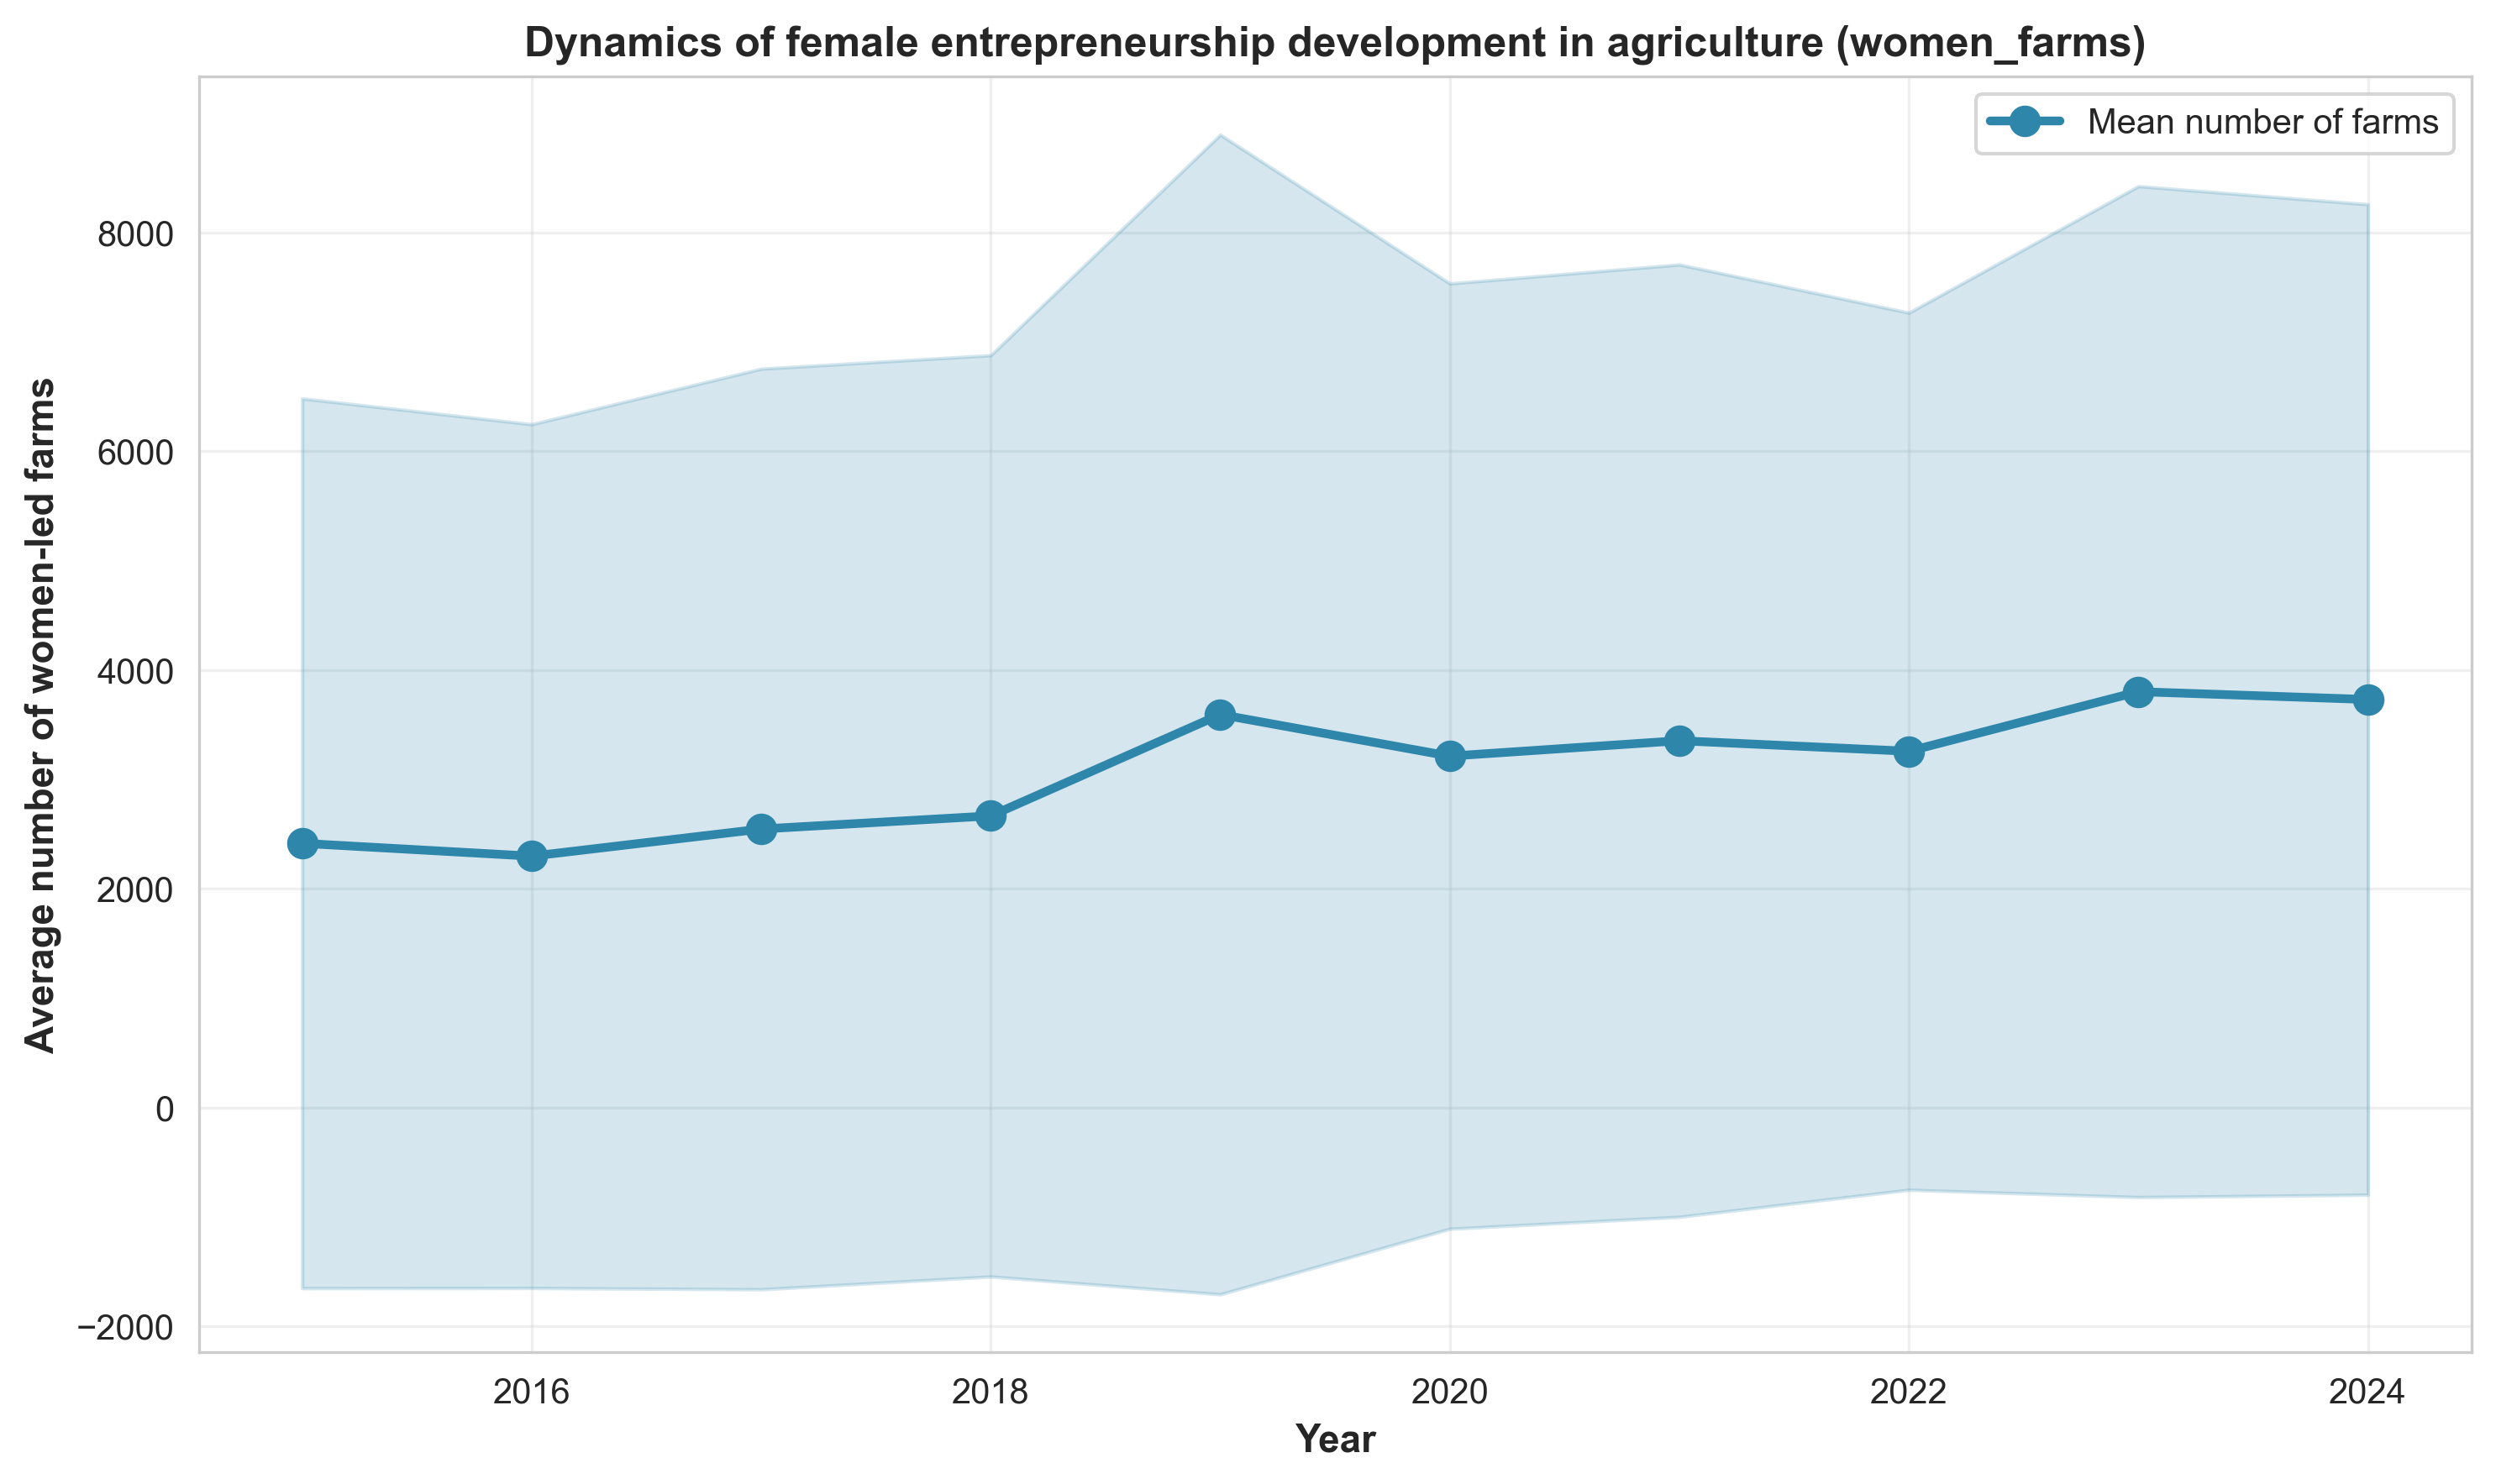
\includegraphics[keepaspectratio]{article_scopus/media/image2.png}}

Figure 1. Average number of women-owned farms, by region of Kazakhstan,
2015--2024

Although the volume of loans increased from 3 billion tenge to 4.5
billion tenge, this growth was concentrated in regions with more
developed infrastructure (Figure 2). Econometric analysis confirms this
conclusion. Pooled OLS summary data shows a positive correlation between
the number of farms owned by women and the volume of loans. However,
when accounting for regional fixed effects using TWFE, this correlation
disappears. The main conclusion is that financial institutions such as
Kazagrofinance, the Agrarian Credit Corporation, and the Agricultural
Financial Support Fund focus on supporting developed regions.

\pandocbounded{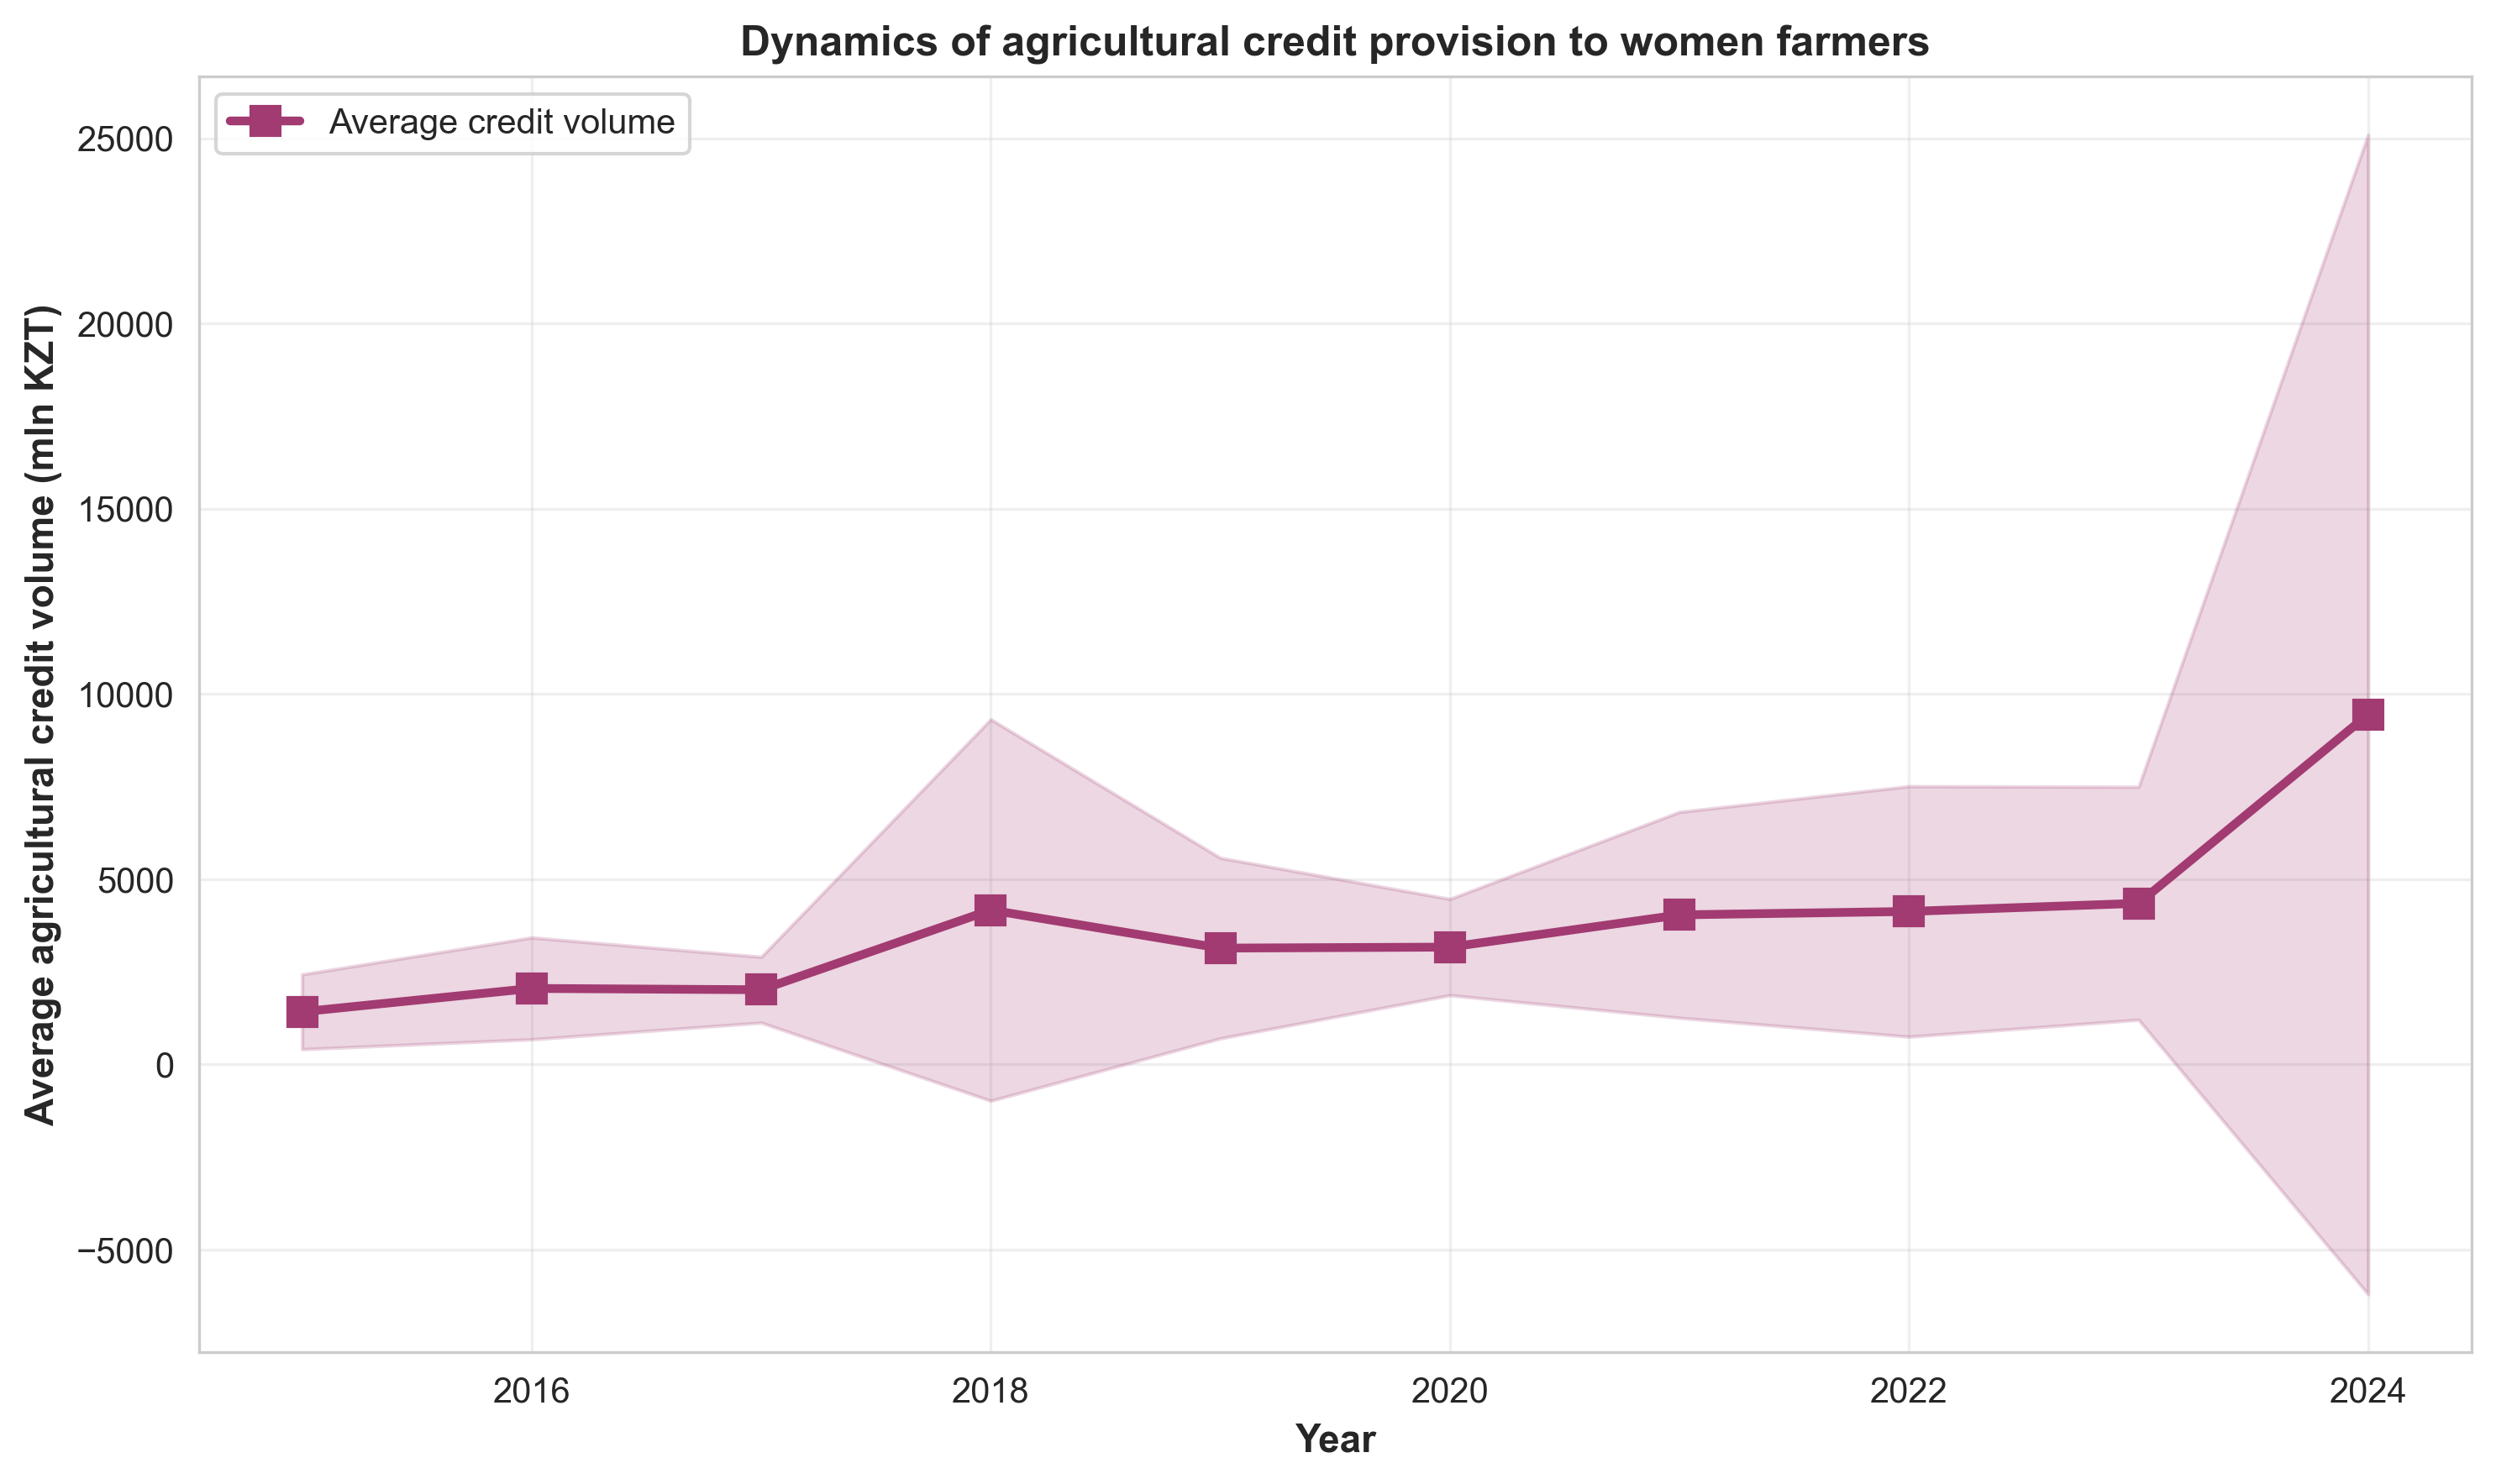
\includegraphics[keepaspectratio]{article_scopus/media/image3.png}}

Figure 2. Volume of loans issued to women farmers

The scatter plot (Figure 3) shows a significant correlation between the
volume of institutional lending and the number of farms owned by women
(r = 0.576, p \textless{} 0.001). Regions with high levels of lending
are characterized by a large number of farms. Estimation of the two-way
fixed-effects (TWFE) model showed that after accounting of regional
differences, the coefficient of the lending variable decreased from
0.725 to 0.044 and lost statistical significance (p = 0.576). This
implies that lending flows to developed regions but does not stimulate
women's entrepreneurship within those regions. This raises the question:
are loans effective, or are there other factors at play?

\pandocbounded{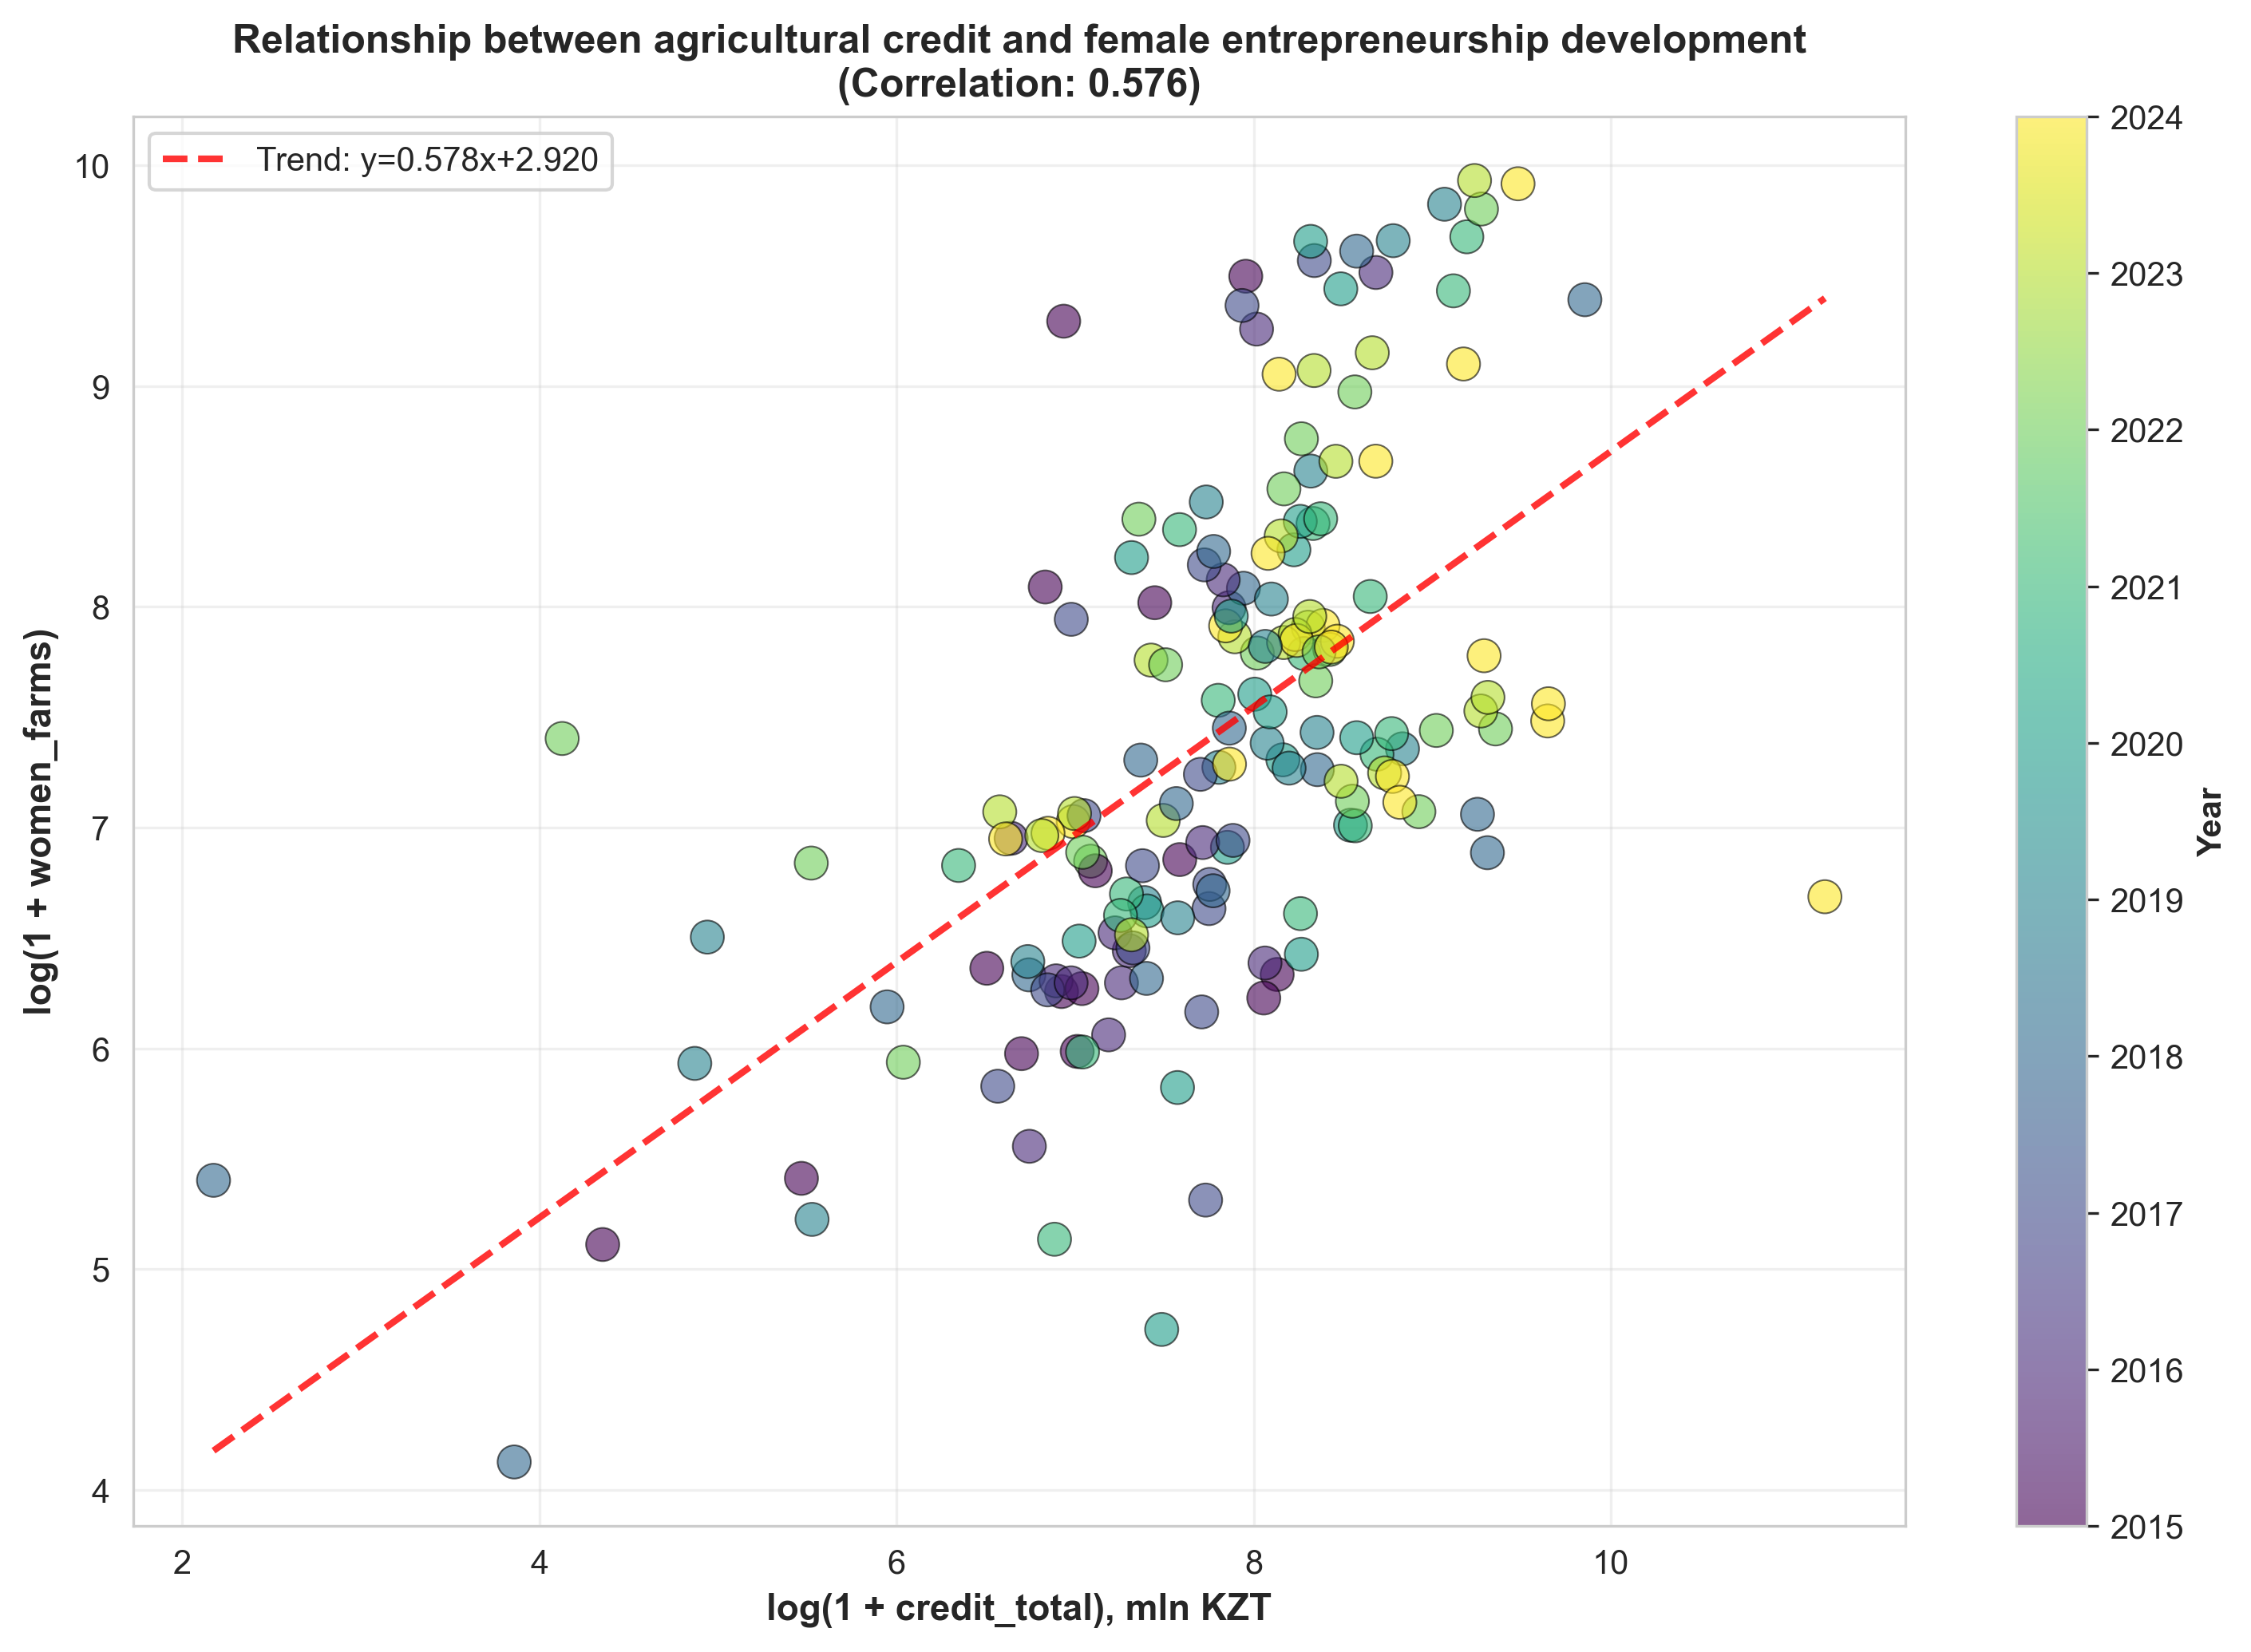
\includegraphics[keepaspectratio]{article_scopus/media/image4.png}}

Figure 3. The relationship between lending and women's entrepreneurship
in agriculture

Correlation analysis alone does not allow us to draw conclusions about
the causal nature of this relationship. The observed relationship may
reflect the influence of third factors, such as the region's level of
economic development, the quality of the institutional environment, or
the availability of infrastructure. In our view, the observed
correlation can be explained by other regional factors or by a feedback
mechanism, whereby the growth of women's entrepreneurship increases the
demand for loans.

4.2 Panel regression results: econometric analysis

Table 2. Comparison of Pooled OLS and TWFE

{\def\LTcaptype{none} % do not increment counter
\begin{longtable}[]{@{}
  >{\raggedright\arraybackslash}p{(\linewidth - 8\tabcolsep) * \real{0.2465}}
  >{\raggedright\arraybackslash}p{(\linewidth - 8\tabcolsep) * \real{0.1975}}
  >{\raggedright\arraybackslash}p{(\linewidth - 8\tabcolsep) * \real{0.1834}}
  >{\raggedright\arraybackslash}p{(\linewidth - 8\tabcolsep) * \real{0.1893}}
  >{\raggedright\arraybackslash}p{(\linewidth - 8\tabcolsep) * \real{0.1834}}@{}}
\toprule\noalign{}
\begin{minipage}[b]{\linewidth}\raggedright
Variable
\end{minipage} & \begin{minipage}[b]{\linewidth}\raggedright
Pooled OLS
\end{minipage} & \begin{minipage}[b]{\linewidth}\raggedright
\end{minipage} & \begin{minipage}[b]{\linewidth}\raggedright
TWFE
\end{minipage} & \begin{minipage}[b]{\linewidth}\raggedright
\end{minipage} \\
\midrule\noalign{}
\endhead
\bottomrule\noalign{}
\endlastfoot
& Coefficient & Standard Error & Coefficient & Standard Error \\
log\_credit\_total & 0.7250*** & (0.0901) & 0.0443 & (0.0834) \\
land\_share & 0.0566* & (0.0341) & 0.0181 & (0.0289) \\
Constant & 1.7143** & (0.6916) & - & - \\
& & & & \\
Model Statistics & & & & \\
N & 149 & & 149 & \\
R² & 0.336 & & 0.030 (within) & \\
Adjusted R² & 0.327 & & 0.099 (overall) & \\
Fixed Effects & No & & Region + Year & \\
SE Type & HC1-robust & & Clustered (region) & \\
\end{longtable}
}

We constructed a panel regression model to assess the impact of
institutional lending on the development of women-owned farms.

Stage 1: Ordinary least squares (Pooled OLS)

The pooled ordinary least squares (OLS) method revealed a positive
correlation between total credit volume and the number of female-headed
farms. The coefficient for the log\_credit\_total variable was 0.725 (p
\textless{} 0.001). This is explained by the fact that a 1\% increase in
credit leads to a 0.73\% increase in the number of female-headed farms.
R² = 0.336, meaning the model explains 33.6\% of the interregional
variation in the dependent variable. The land access variable
land\_share is also significant at the 10\% level, confirming the
importance of land rights for women.

The Pooled OLS model showed that the higher the volume of lending, the
greater the number of farms. However, this is because these regions
initially have better infrastructure and access to the loans. In other
words, the specification of this model does not account for these
regional characteristics.

Stage 2. TWFE Fixed-effects model

To account for these differences, we applied the TWFE fixed-effects
model, which incorporates these regional characteristics. Here, we
observe that the coefficient for the credit variable decreases from
0.725 to 0.044 and loses statistical significance (p = 0.596).

The following conclusions can be drawn: the second TWFE model primarily
reflects interregional differences, meaning that loans are initially
concentrated in regions with higher levels of women's entrepreneurship
rather than stimulating its growth in regions. This finding further
confirms the hypothesis that financial instruments are unable to
stimulate the growth of women's entrepreneurship without corresponding
institutional reforms, including expanding women's access to land.

\pandocbounded{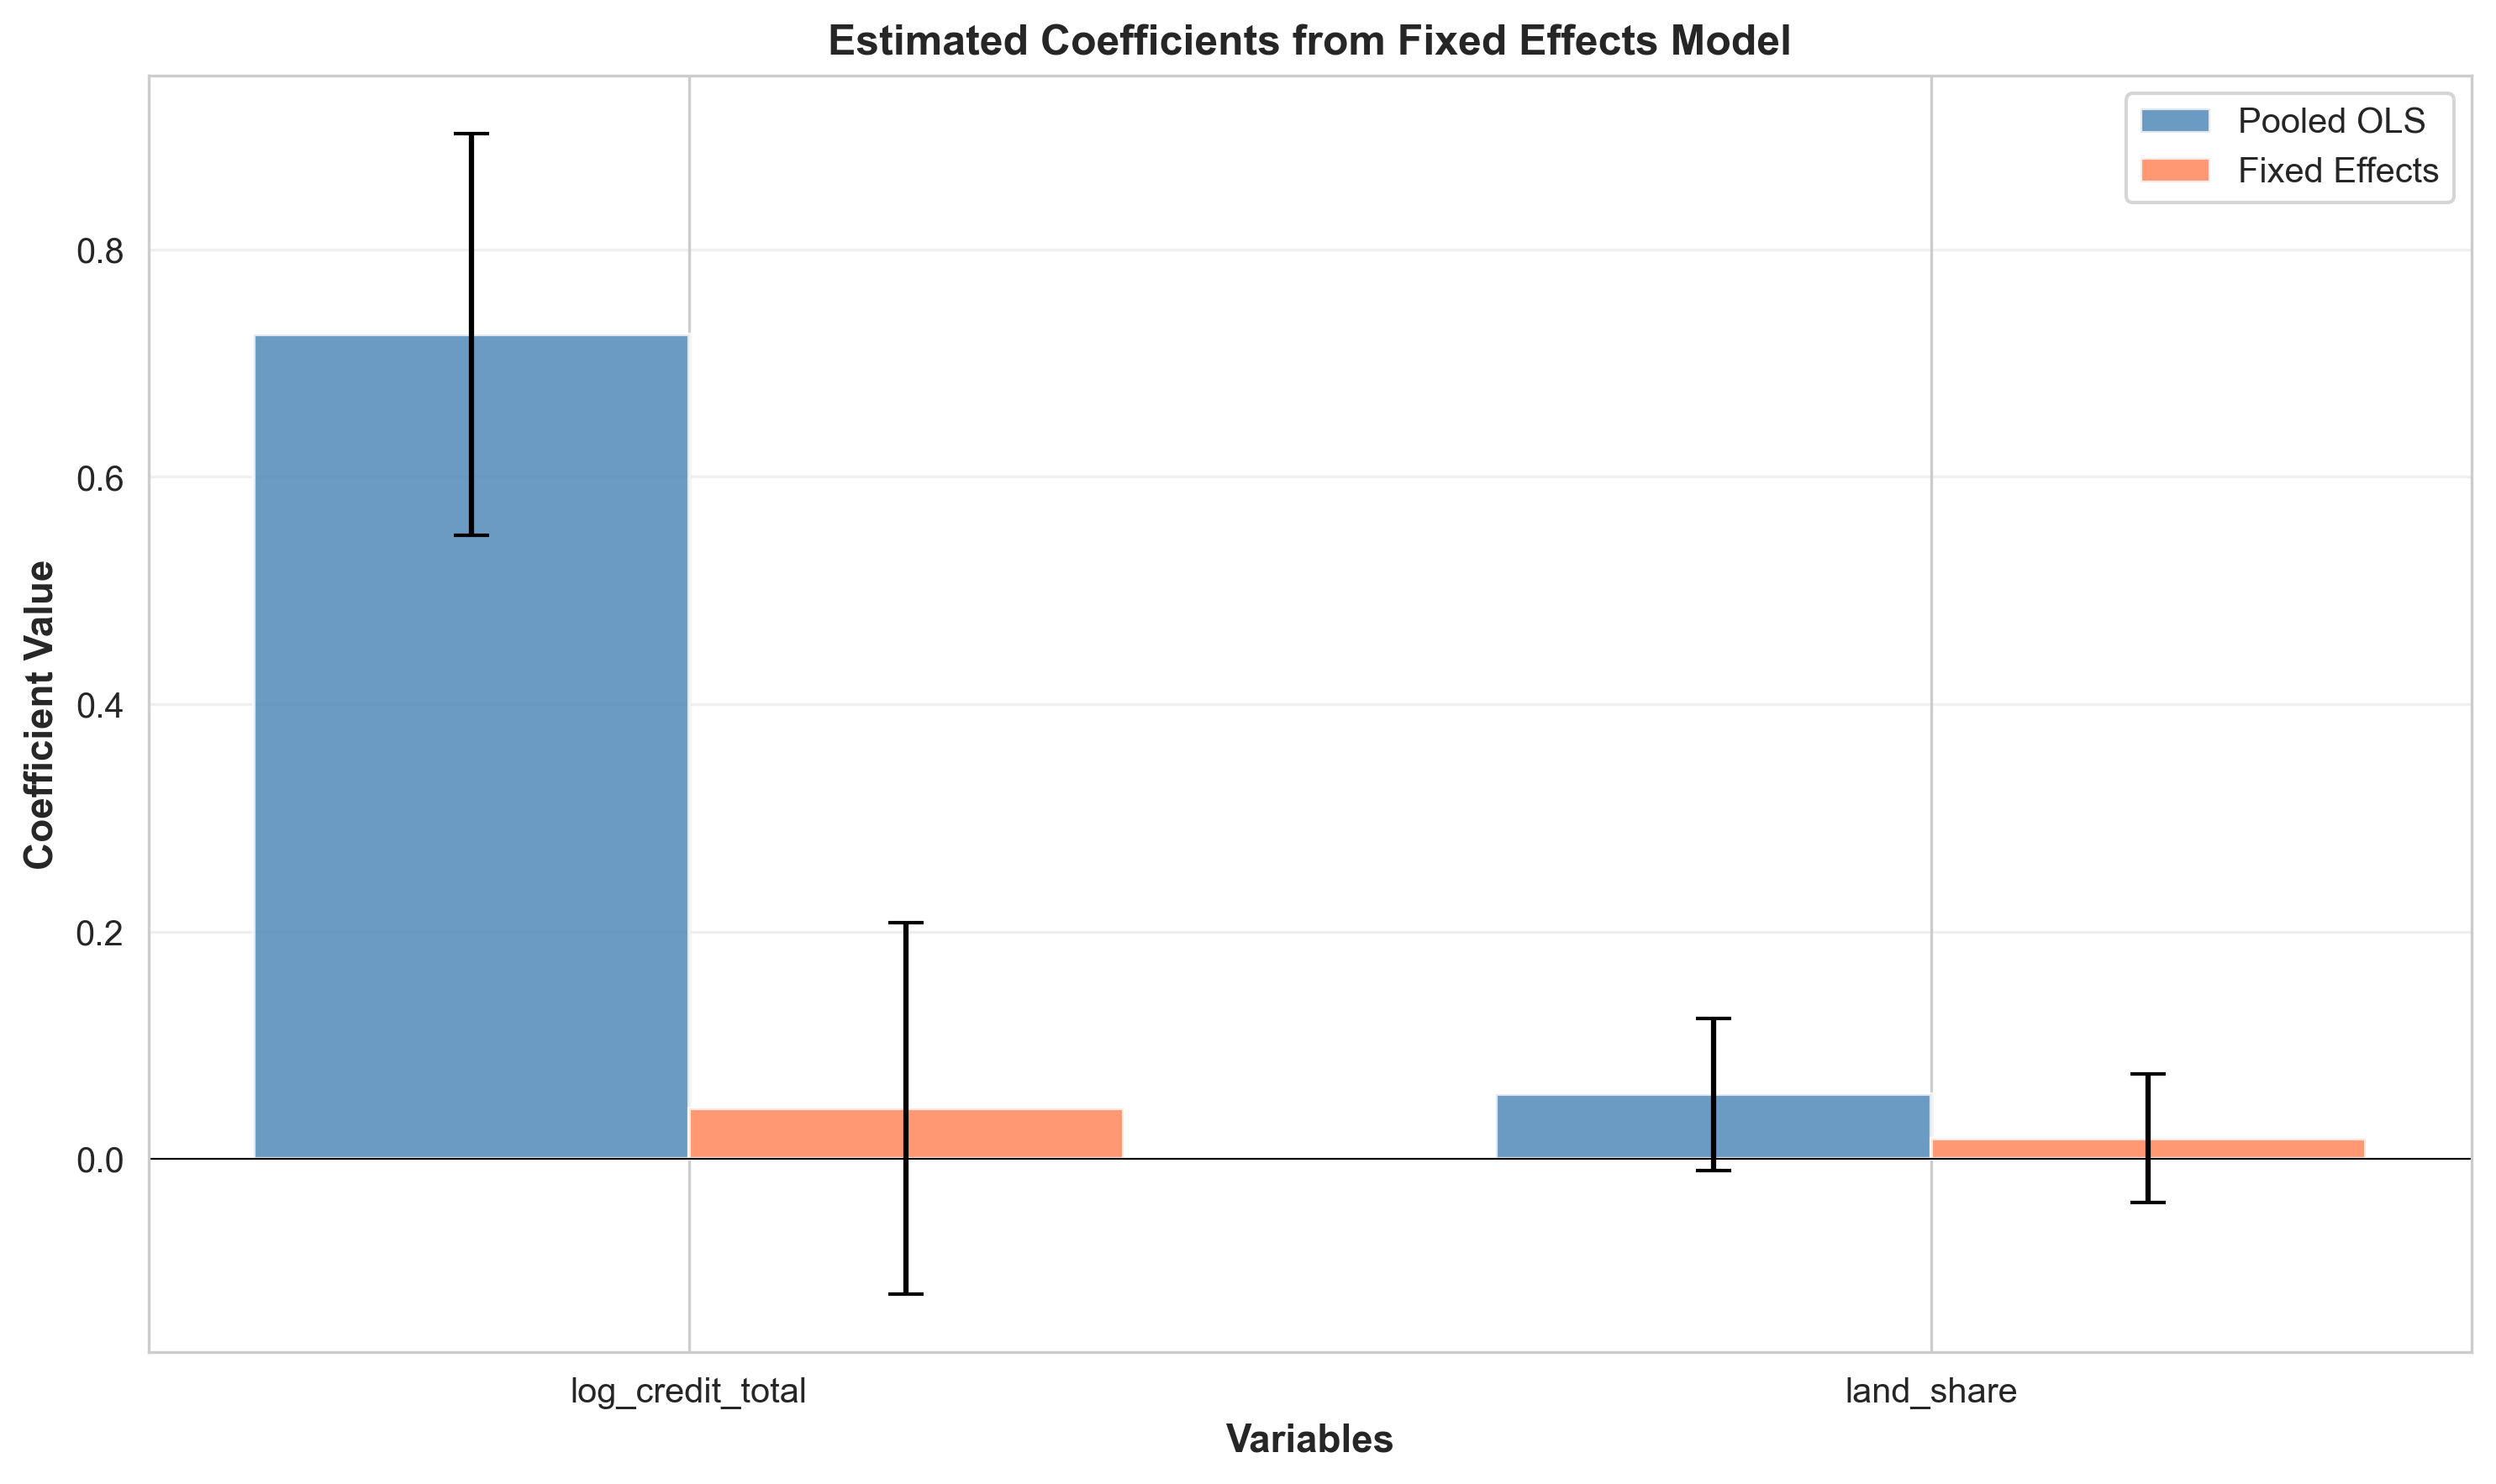
\includegraphics[keepaspectratio]{article_scopus/media/image5.png}}

Figure 4. Comparison of the Pooled OLS and TWFE models

Figure 4 clearly shows that in the Pooled OLS model, the credit
coefficient is positive at 0.725 (p \textless{} 0.001) and significant.
In the TWFE model, it is practically zero (0.0443) and crosses the zero
line on the graph. This confirms that the observed interregional
correlation is due to interregional differences, rather than the impact
of lending on women's entrepreneurship.

Stability test by decomposing lending into sources

We replaced the aggregate lending indicator with three components: loans
from Kazagrofinance JSC, Agrarian Credit Corporation JSC, and the
Agricultural Financial Support Fund JSC

Table 3 Results of the model estimation by lending source

{\def\LTcaptype{none} % do not increment counter
\begin{longtable}[]{@{}
  >{\raggedright\arraybackslash}p{(\linewidth - 10\tabcolsep) * \real{0.1897}}
  >{\raggedright\arraybackslash}p{(\linewidth - 10\tabcolsep) * \real{0.1823}}
  >{\raggedright\arraybackslash}p{(\linewidth - 10\tabcolsep) * \real{0.1663}}
  >{\raggedright\arraybackslash}p{(\linewidth - 10\tabcolsep) * \real{0.1617}}
  >{\raggedright\arraybackslash}p{(\linewidth - 10\tabcolsep) * \real{0.1576}}
  >{\raggedright\arraybackslash}p{(\linewidth - 10\tabcolsep) * \real{0.1425}}@{}}
\toprule\noalign{}
\begin{minipage}[b]{\linewidth}\raggedright
Variable
\end{minipage} & \begin{minipage}[b]{\linewidth}\raggedright
Coefficient
\end{minipage} & \begin{minipage}[b]{\linewidth}\raggedright
Standard error
\end{minipage} & \begin{minipage}[b]{\linewidth}\raggedright
t-statistic
\end{minipage} & \begin{minipage}[b]{\linewidth}\raggedright
p-value
\end{minipage} & \begin{minipage}[b]{\linewidth}\raggedright
N
\end{minipage} \\
\midrule\noalign{}
\endhead
\bottomrule\noalign{}
\endlastfoot
log\_credit\_kaf & 0.0031 & (0.0365) & 0.084 & 0.933 & 88 \\
log\_credit\_acc & -0.0473 & (0.0484) & -0.979 & 0.331 & 88 \\
log\_credit\_fund & -0.0073 & (0.0647) & -0.113 & 0.910 & 88 \\
\end{longtable}
}

The calculations presented in Table 3 show that none of the three
sources of lending had a statistically significant effect, while the
sample size was reduced to 88 observations due to missing data on
lending from the Agricultural Financial Support Fund. The coefficients
are close to zero, ranging from -0.473 to 0.003, and the p-values exceed
0.05 (0.933, 0.331, and 0.910). These calculations demonstrated once
again that credit flows do not influence the formation of female-headed
households (data from the main TWFE model)

4.3 Regional clustering

To identify regional heterogeneity in the characteristics of women's
entrepreneurship development, the k-means clustering method was applied.
Based on seven indicators -- mean values and standard deviations of the
number of women-owned farms and the volume of lending, the share of
land, and the development trend -- regions were grouped into two
clusters (optimality determined by the Silhouette Score criterion =
0.400), table 4

Table 4. Regional cluster profiles

{\def\LTcaptype{none} % do not increment counter
\begin{longtable}[]{@{}
  >{\raggedright\arraybackslash}p{(\linewidth - 10\tabcolsep) * \real{0.1347}}
  >{\raggedright\arraybackslash}p{(\linewidth - 10\tabcolsep) * \real{0.1435}}
  >{\raggedright\arraybackslash}p{(\linewidth - 10\tabcolsep) * \real{0.2250}}
  >{\raggedright\arraybackslash}p{(\linewidth - 10\tabcolsep) * \real{0.1956}}
  >{\raggedright\arraybackslash}p{(\linewidth - 10\tabcolsep) * \real{0.1476}}
  >{\raggedright\arraybackslash}p{(\linewidth - 10\tabcolsep) * \real{0.1536}}@{}}
\toprule\noalign{}
\begin{minipage}[b]{\linewidth}\raggedright
Cluster
\end{minipage} & \begin{minipage}[b]{\linewidth}\raggedright
N regions
\end{minipage} & \begin{minipage}[b]{\linewidth}\raggedright
log\_women\_farms (mean value)
\end{minipage} & \begin{minipage}[b]{\linewidth}\raggedright
log\_credit\_total (mean value)
\end{minipage} & \begin{minipage}[b]{\linewidth}\raggedright
Share of land (average value, \%)
\end{minipage} & \begin{minipage}[b]{\linewidth}\raggedright
Growth trend (annual)
\end{minipage} \\
\midrule\noalign{}
\endhead
\bottomrule\noalign{}
\endlastfoot
Cluster 0 & 15 & 7.71 & 8.02 & 2.30 & 0.091 \\
Cluster 1 & 5 & 6.35 & 6.75 & 0.18 & 0.296 \\
\end{longtable}
}

Note: Average characteristics of regional clusters. Growth trend -- the
slope of the log\_women\_farms linear trend over time, characterizing
the growth rate of women's entrepreneurship.*

Cluster analysis divided the regions into two groups.

Cluster 0 (15 regions) -- rural areas with a high level of women's
farming (log\_women\_farms = 7.71, corresponding to approximately 2,230
farms on average per region), high total credit volume
(log\_credit\_total = 8.02, or about 3,050 million tenge), and a
relatively high share of land owned by women (2.30\%). However, the
growth rate here is moderate: 0.091 logarithms per year, which
translates to about 9.5\% annual growth.

Cluster 1 (5 regions) -- regions with a low starting point. Here, there
are four times fewer women-owned farms (log\_women\_farms = 6.35, about
570 farms), 3.6 times fewer loans (log\_credit\_total = 6.75, about 850
million tenge), and the share of land owned by women is practically zero
(0.18\%). However, the growth rate is three times higher: 0.296
logarithms per year, or about 34.5\% growth per year.

\emph{*Note: Since the dependent variable is taken in natural logarithm,
the linear trend coefficient β corresponds to the approximate growth
rate in percentage terms. For Cluster 0, β = 0.091 yields about 9.5\%
growth per year; for Cluster 1, β = 0.296 yields about 34.5\% per
year.*}

According to our calculations, these results are significant for two
reasons. First, rapid growth in regions with low levels of lending
suggests that loans are not the driving force. The dynamics of women's
farming are not determined by the current volume of loans or the
availability of land. Regions with the least initial opportunities
demonstrate the greatest growth potential, while more developed regions
are experiencing a saturation effect.

The results are consistent with the findings of fixed-effects models.

\pandocbounded{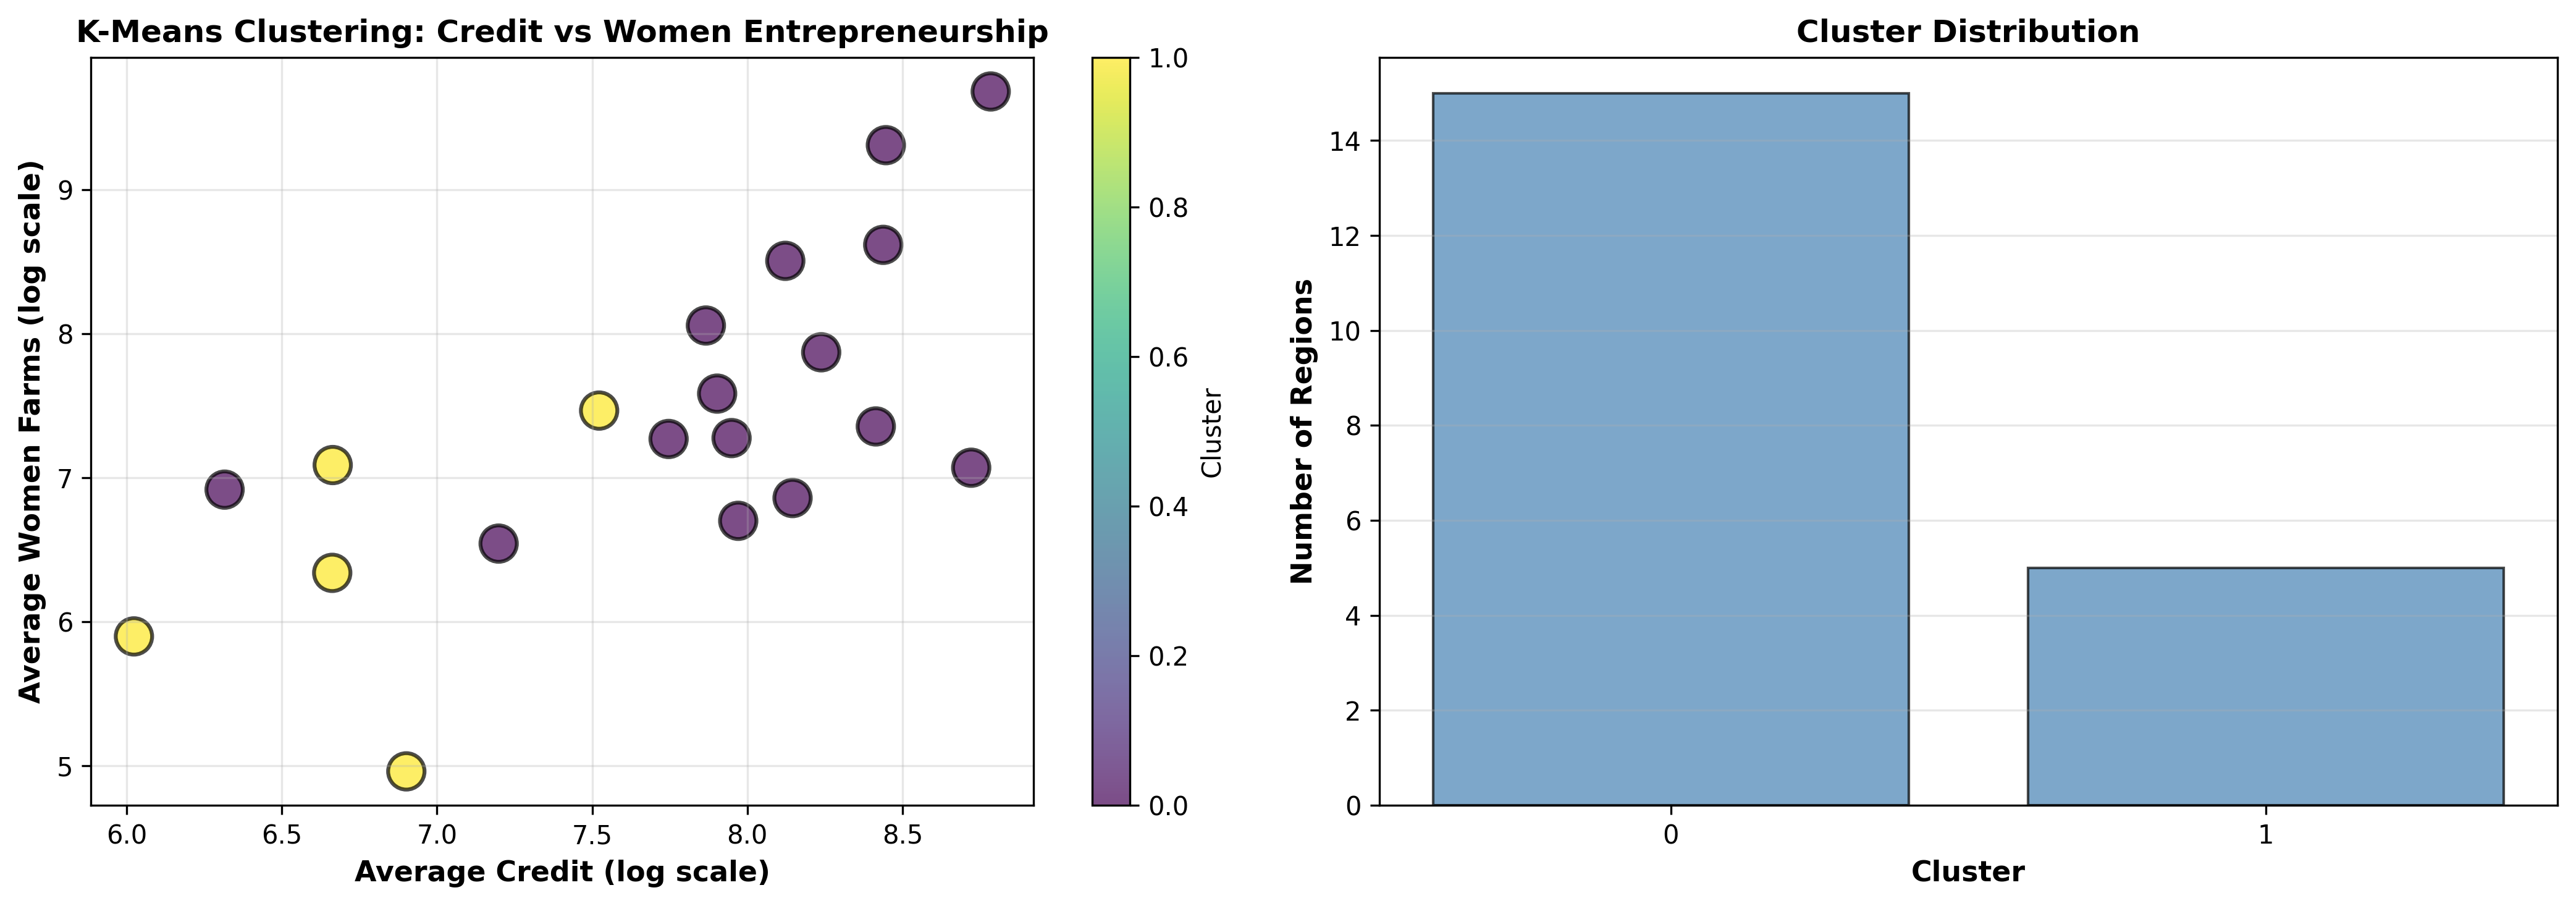
\includegraphics[keepaspectratio]{article_scopus/media/image6.png}}

Figure 5. Regional clusters based on lending and women's
entrepreneurship

In the scatter plot, Cluster 0 (blue) is located in the high-value are
along both the lending axis and the women's entrepreneurship axis, while
Cluster 1 (yellow) is in the lower-value area for both characteristics.
Regions with a low baseline but high growth potential (cluster 1)
require different measures than regions where the women's agribusiness
sector is already developed (cluster 0). In our opinion, for the first
group of regions in Kazakhstan, the priority may be the removal of
institutional barriers (access to land, infrastructure), while for the
second group, it may be improving efficiency and diversification.

4.4 Analysis of features' importance: Random Forest

To understand which variables best influence the development of women's
farming and to check for nonlinear relationships, we used the Random
Forest method. The model was trained using group cross-validation
(GroupKFold, 5 folds per region). This ensures that data from the same
region are not included in both the training and test sets.

Table 5. Feature Importance from the Random Forest Model

{\def\LTcaptype{none} % do not increment counter
\begin{longtable}[]{@{}
  >{\raggedright\arraybackslash}p{(\linewidth - 4\tabcolsep) * \real{0.3372}}
  >{\raggedright\arraybackslash}p{(\linewidth - 4\tabcolsep) * \real{0.3323}}
  >{\raggedright\arraybackslash}p{(\linewidth - 4\tabcolsep) * \real{0.3306}}@{}}
\toprule\noalign{}
\begin{minipage}[b]{\linewidth}\raggedright
Feature
\end{minipage} & \begin{minipage}[b]{\linewidth}\raggedright
Importance
\end{minipage} & \begin{minipage}[b]{\linewidth}\raggedright
\% Total
\end{minipage} \\
\midrule\noalign{}
\endhead
\bottomrule\noalign{}
\endlastfoot
log\_credit\_fund & 0.448 & 44.76\% \\
log\_credit\_total & 0.146 & 14.56\% \\
log\_credit\_acc & 0.102 & 10.23\% \\
lag1\_log\_credit\_total & 0.102 & 10.22\% \\
land\_share & 0.088 & 8.84\% \\
log\_credit\_kaf & 0.082 & 8.19\% \\
year & 0.032 & 3.20\% \\
\end{longtable}
}

We used a Random Forest model to identify the variables that best
predict the development of women's agriculture and to test for nonlinear
relationships that are not detected by linear models. We also used group
cross-validation to assess the model's quality.

The data in table 5 shows that loans provided through the Agricultural
Financial Support Fund account for the largest share at 44.8\%. Total
loans rank second at 14.6\%, nearly three times smaller. This
demonstrates the importance of the funding source and that not all loans
are effective. It is crucial to distinguish loans by source; that is,
the effectiveness of loans is determined by the source, not the volume.
Systematic changes over the years do not affect the dependent variable.
Land is also important for the sustainable development of agriculture
and women's entrepreneurship (8.84\%).

The Random Forest model showed that the variables can accurately predict
outcomes and confirms a significant correlation between loans and women
farmers. The TWFE model, on the other hand, estimates the change in the
outcome when each factor changes. This suggests that loans are
concentrated in areas where women's entrepreneurship was already
developed. This distinction between correlation and causation is the
result of our study.

\pandocbounded{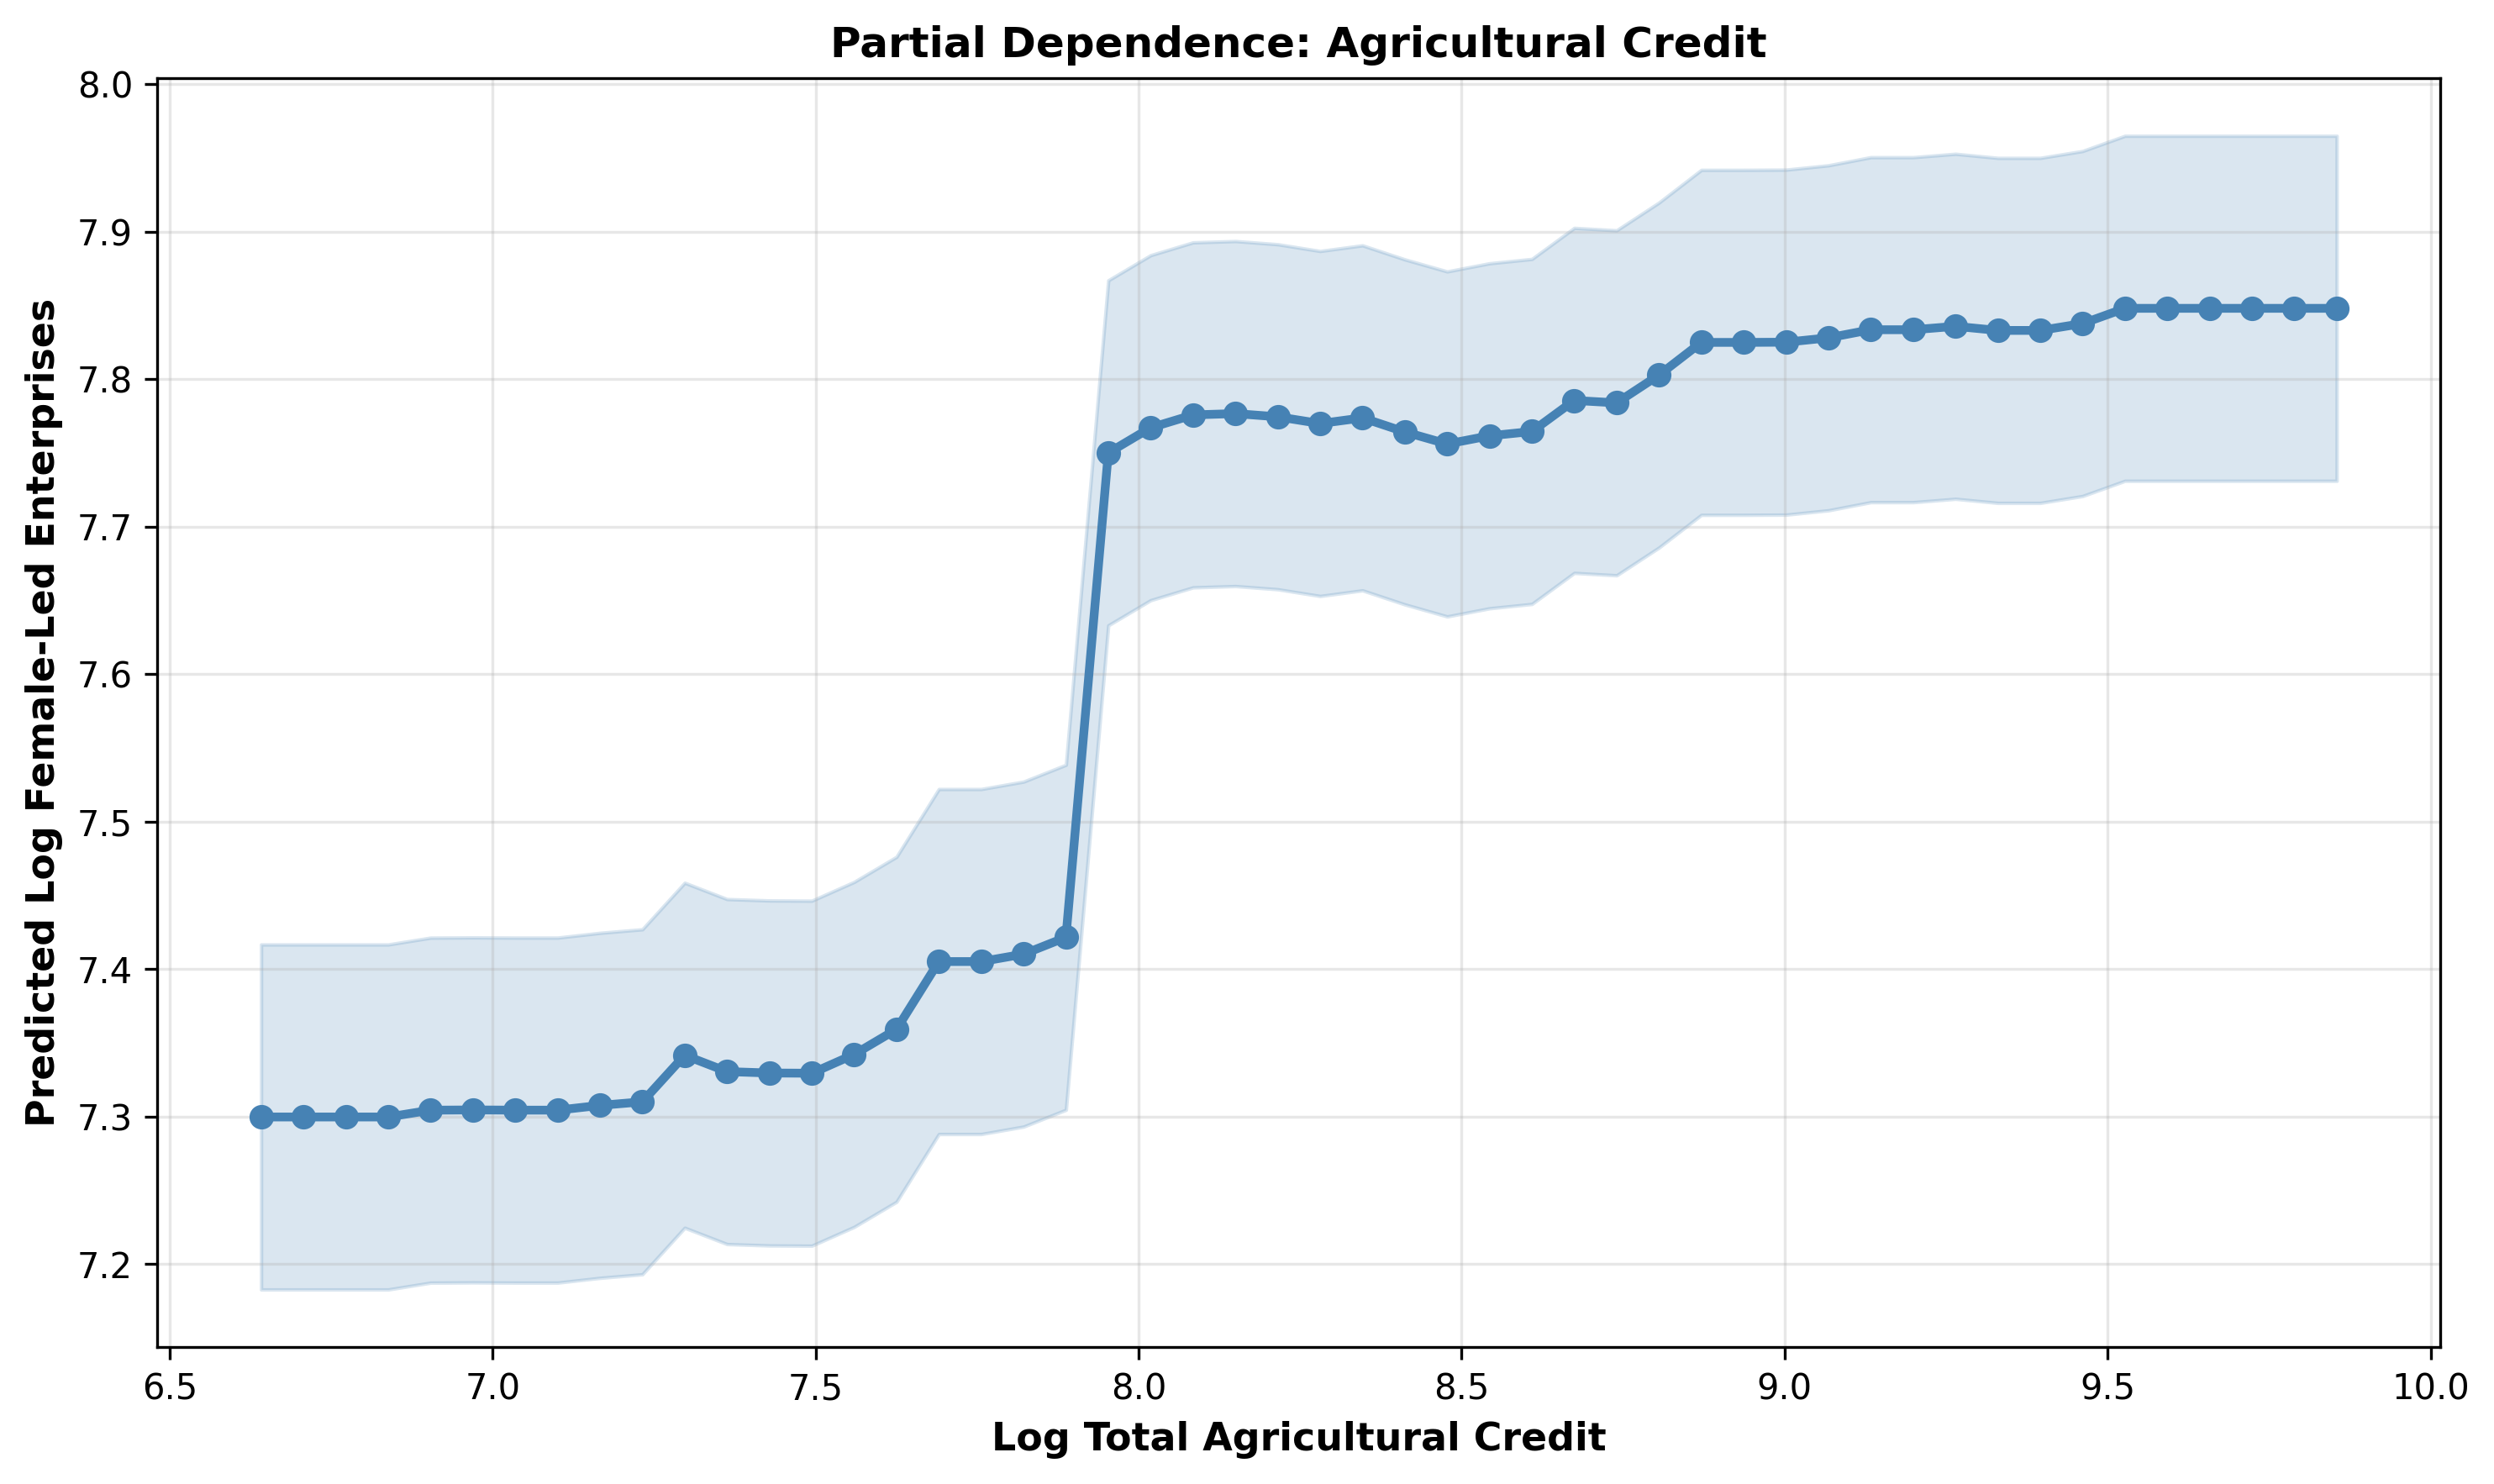
\includegraphics[keepaspectratio]{article_scopus/media/image7.png}}

Figure 6. Relationship between loan amount and the number of farms owned
by women

The graph generated using the Random Forest model (Figure 6) shows a
positive correlation between loan amount and the predicted number of
farms owned by women. The absence of a significant effect in the TWFE
model indicates that the relationship observed in Figure 6 is driven by
the structural characteristics of the regions, rather than a causal
effect of loans.

\pandocbounded{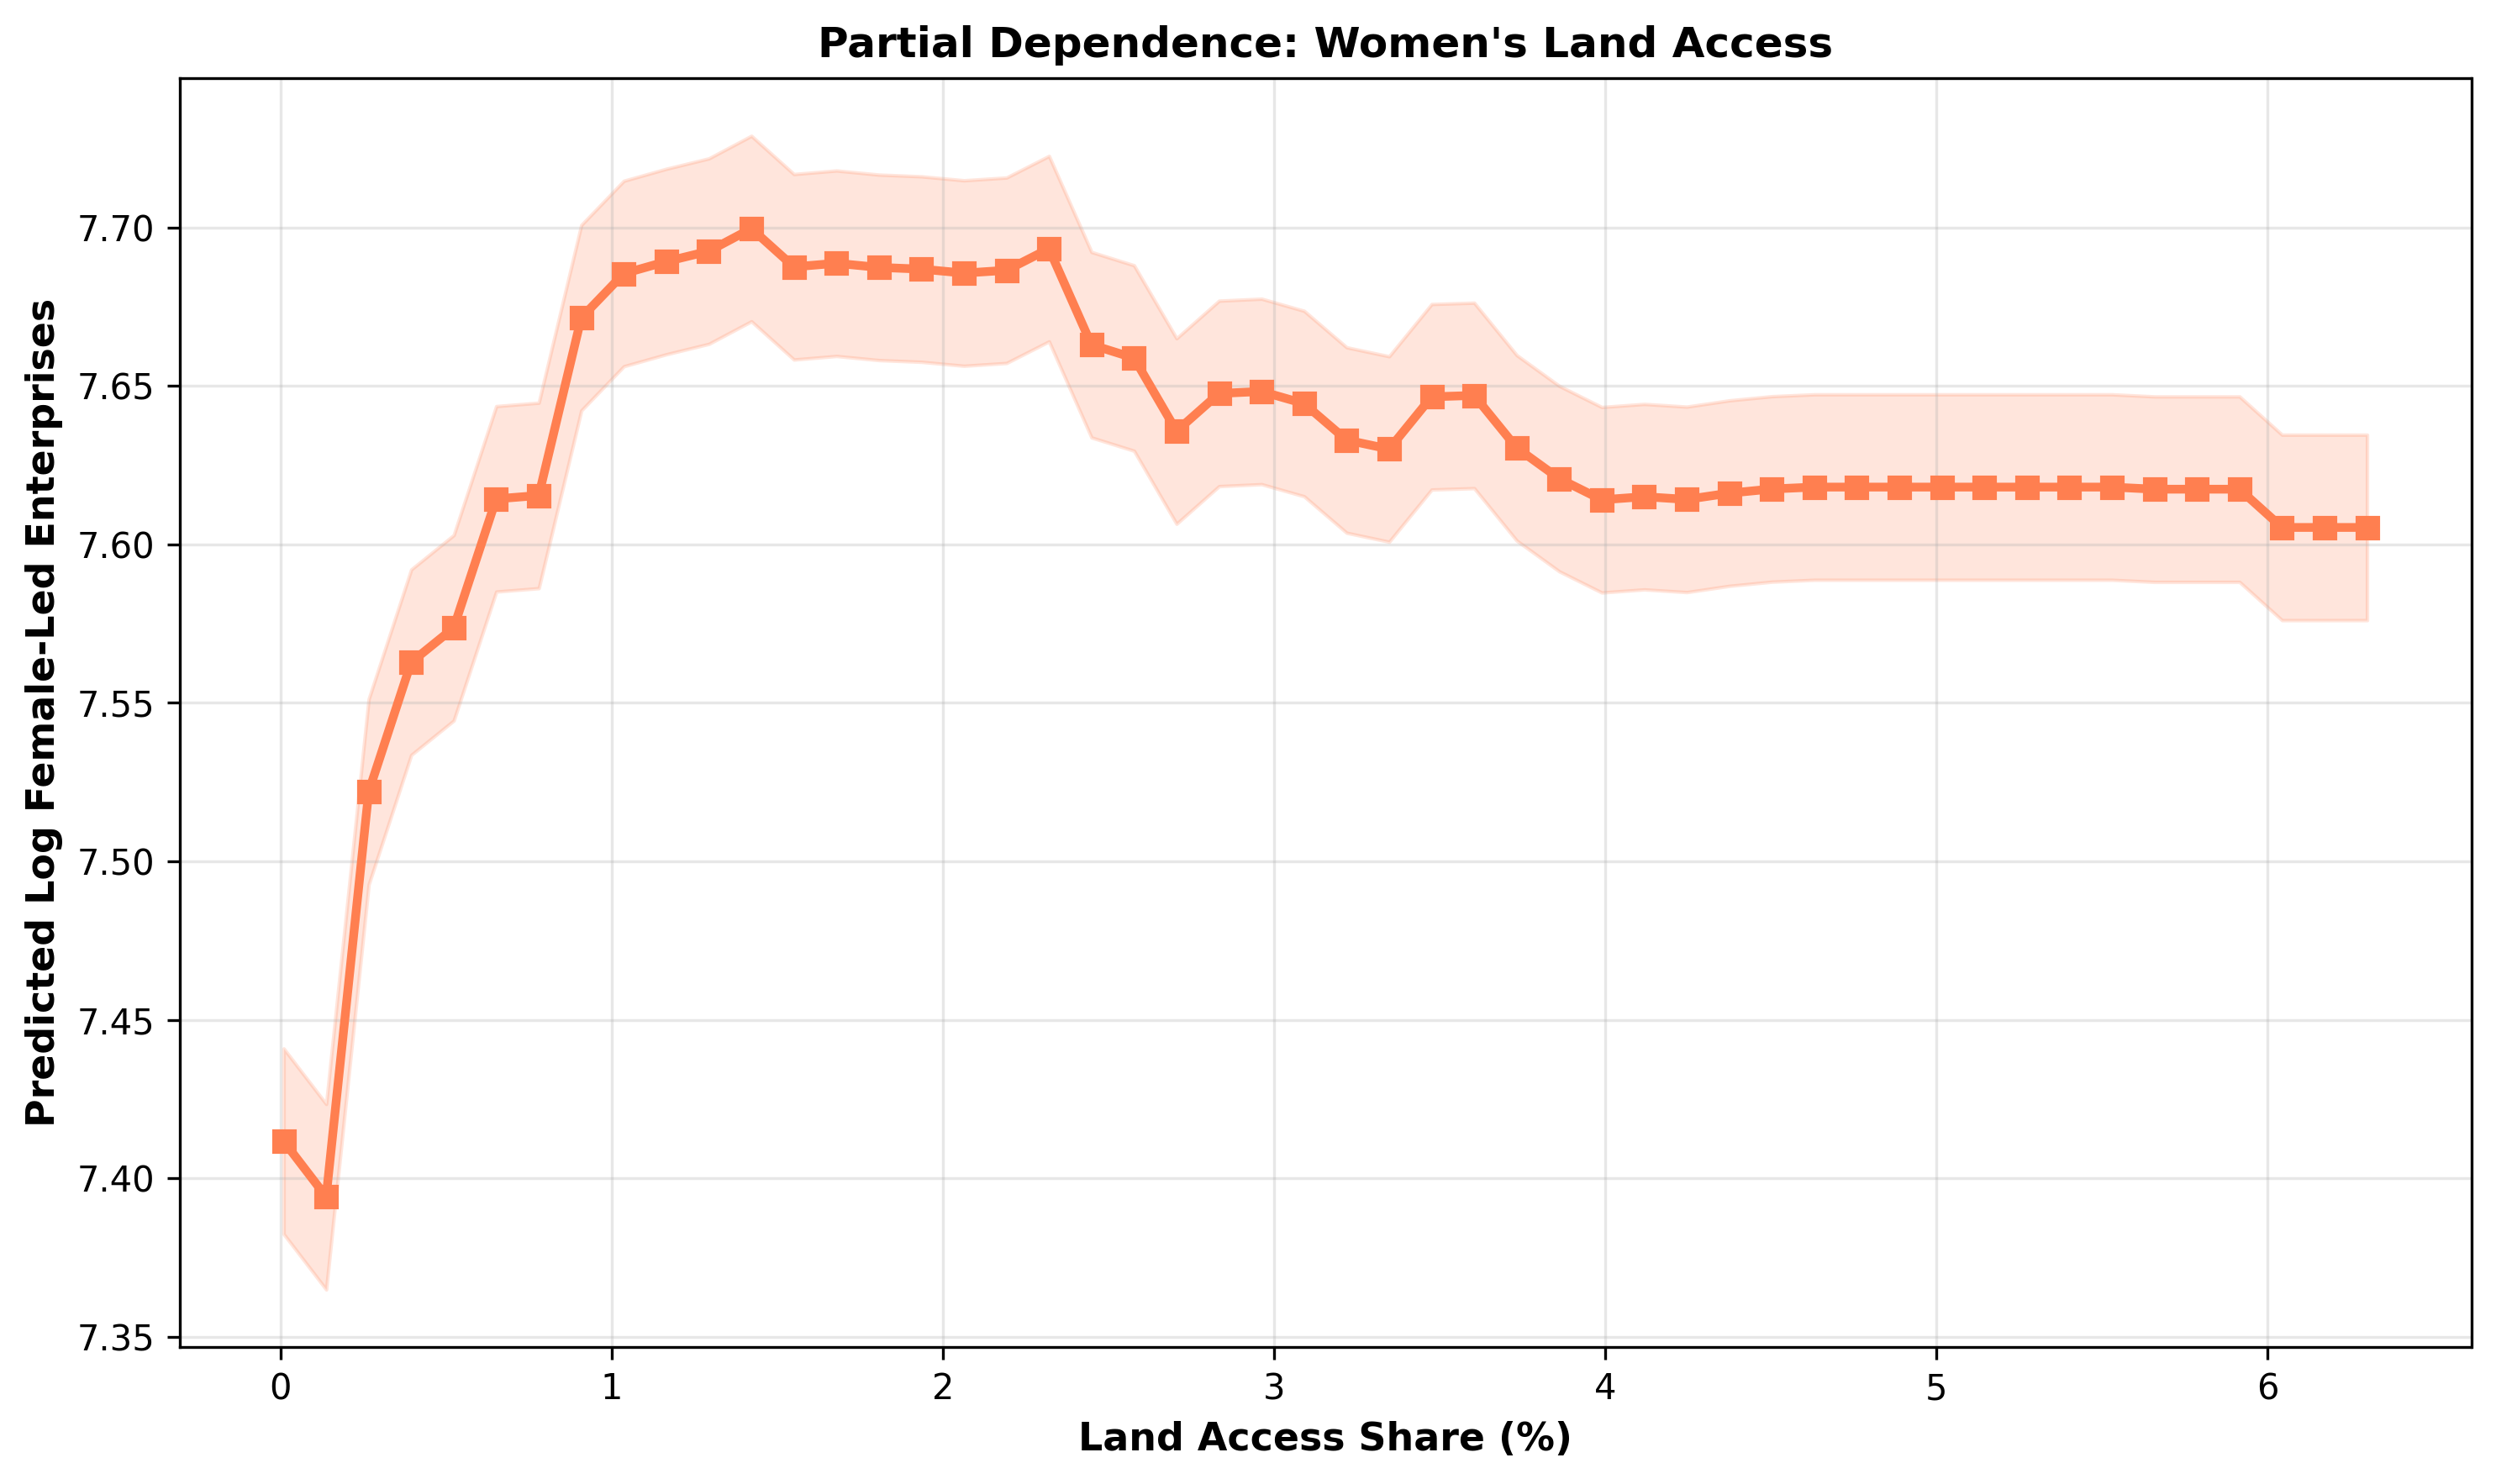
\includegraphics[keepaspectratio]{article_scopus/media/image8.png}}

Figure 7. Relationship between access to land and the number of
women-owned farms

Figure 7 shows a nonlinear relationship between land ownership and the
predicted number of farms owned by women, which is consistent with the
hypothesis \hl{(Lin \& Peng, 2025; Han \& Zhang, 2026, and Ye,
2025\textbf{)}.} This relationship is weakly positive up to 2\%,
stabilizes in the range from 2\% to 6\%, and increases again above 6\%.
For Kazakhstan, this means that to enhance the impact of lending, it is
necessary to overcome the 2\% threshold in land ownership. Overcoming
this barrier will lead to a multiplier effect and the use of land as a
financial asset (consistent with the ``critical minimum of assets''
hypothesis for entrepreneurial activity\hl{,} \hl{Carter, 2022).}

However, the quality of the Random Forest model was low: RMSE = 0.95, R²
= --0.56. The negative coefficient of determination indicates that the
model predicts worse than the simple average. This suggests that the
Random Forest model cannot adequately capture regional characteristics
without introducing fixed effects. This confirms our main conclusion
that lending is not the cause of the growth in the number of farms owned
by women. Consequently, a more complex model, such as TWFE, is needed,
one that accounts for regional heterogeneity and demonstrates that
lending has no impact on the development of farms owned by women.

An analysis of panel data for 20 regions of Kazakhstan covering the
years 2015--2024 reveals several key findings.

1. Lending does not have a negative impact on the growth in the number
of farms owned by women. A simple Pooled OLS model shows a positive
relationship: a 1\% increase in lending is associated with a 0.73\%
increase in the number of farms (p \textless{} 0.001). When applying
time- and region-fixed effects (TWFE), the coefficient drops to 0.044,
meaning it becomes insignificant (p = 0.596). Consequently, the
correlation we observed is not explained by the fact that loans support
women's businesses in Kazakhstan, but rather by the fact that they are
primarily directed toward more developed regions.

2. The result is robust. We disaggregated the loans by source
(KazAgroFinance, Agrarian Credit Corporation, Financial Support Fund),
but none yielded a significant effect. The sample under study was
reduced to 88 observations (there is less data for the Financial Support
Fund), but all three components yielded the same result. These results
showed that lending does not play a significant role in the emergence of
new women-owned farms.

3. Access to land as an institutional factor in the successful
development of women's entrepreneurship in agriculture. The share of
land held by women farmers averages just 2.01\% (median 1.19\%), and in
some regions it is close to zero. This finding indicates that without
resolving the issue of access to land, credit support alone cannot
stimulate the growth of women's entrepreneurship in Kazakhstan's
agricultural sector.

4. Two clusters of rural development. Cluster analysis (k-means)
revealed a consistent division of regions into two groups. Cluster 0 (15
regions) is characterized by a high level of women's farming
(log\_women\_farms = 7.71) and lending (log\_credit\_total = 8.02). It
has relatively higher access to land for women farmers (2.3\%), but a
moderate growth rate of 9.5\% per year. Cluster 1 (5 regions) exhibits
low baseline levels (log\_women\_farms = 6.35, log\_credit\_total =
6.75), extremely limited access to land (0.18\%), but growth of
approximately 34.5\% per year. Regions with low starting levels are
characterized by rapid growth, but this growth is not linked to the
current volume of loans, which also remains low in these regions
(confirming the absence of a uniform lending effect in TWFE).

5. Loans effectively support but do not influence the development of
agriculture in Kazakhstan. Analysis using the Random Forest method
showed that variables related to loans explain 87.9\% of the model's
predictive power. Loans from the Financial Support Fund are particularly
significant (44.8\%). The partial dependency graphs confirm that the
more loans there are, the higher the predicted number of female-headed
farms. However, the model generalizes poorly to the newly formed regions
of Kazakhstan (R² = --0.56). In other words, loans effectively explain
in which regions there are more farms (interregional differences), but
they do not explain why they are growing (intraregional dynamics). Our
calculations showed that loans are concentrated in regions where women's
agriculture was initially well-developed.

6. Implications of the results for improving agricultural policy in
Kazakhstan. The findings have direct implications for Kazakhstan's
agricultural policy and demonstrate the ineffectiveness of universal
approaches in supporting women's entrepreneurship. A broad expansion of
lending without taking into account structural regional differences and
institutional barriers (especially access to land) will not lead to an
increase in women's entrepreneurship in agriculture.

5. Discussion of the results

5.1. Interpretation of key findings: lending constraints

The main finding of the study is a comparison of the estimates obtained
using the Pooled OLS and TWFE models. While the first specification
shows a statistically significant positive effect of lending, the second
demonstrates that this effect disappears entirely after controlling for
fixed effects of region and year. This observation is consistent with
the institutional approach to sector development (\hl{Quisumbing et al.,
2023; Schoneveld \& Weng, 2023}). Loans, provided mainly in areas with a
high share of women entrepreneurs, do not contribute to the creation of
new farms. This is confirmed by data obtained using two additional
analytical methods.

1. Cluster analysis identified two types of regions: developed regions
with high levels of female entrepreneurship and access to loans (15
regions) and less developed regions (5 regions) with high growth rates.
In both groups, the level of lending does not determine growth trends.

2. Random Forest analysis confirmed that variables characterizing
lending are indicators of regional differences; however, the negative
correlation coefficient (R²) from cross-validation showed that
unobserved regional characteristics predominate. Taken together, the
data confirms hypothesis H1: the observed correlations reflect the
structural heterogeneity of regions (between variables) rather than a
causal effect of lending on intra-regional dynamics (within variables).

5.2. Research results. So, why don't loans work?

The main finding of the study that we wish to highlight is the
discrepancy between the two models: Pooled OLS (with a credit
coefficient of 0.725) and the TWFE model (0.044). The first shows a
positive effect of loans, while the second shows their complete
disappearance after accounting for differences between regions
(geography, climate, infrastructure) and time-fixed effects (price
increase, changes in government development programs, macroeconomic
trends, and others). This observation, consistent with the institutional
approach to inclusive development (\hl{Quisumbing et al., 2023;
Schoneveld \& Weng, 2023}), suggests that the lack of an effect in the
region is due not to the ineffectiveness of lending programs, but to
structural factors.

\hl{Carter (2022)} and \hl{Lin \& Peng (2025)} have shown that digital
financial instruments can reduce transaction costs but are ineffective
without access to human capital and collateral. In Kazakhstan, the share
of women who own land is 2.01\%, which is a critical threshold.

\hl{Issahaku (2024}) reaches a similar conclusion in his study of
digital finance and agriculture: access to financing is a necessary but
insufficient condition. Without accompanying institutional reforms (land
rights, market access, advisory services), lending measures will not
lead to sustainable growth.

Lending is widespread in regions with a developed female
entrepreneurship sector, but it does not contribute to the creation of
new business forms. This is confirmed by data obtained using two
additional analytical methods:

1. Cluster analysis identified two stable regional types in Kazakhstan:
developed regions with high levels of women's entrepreneurship and
access to loans (15 regions) and less developed regions with low
indicators but high growth rates (5 regions) (cluster 1).

2. Lending variables are the most important factors effectively
reflecting differences between regions (Random Forest algorithm).
However, the negative coefficient of determination (R²) from the
cross-validation indicates that unobserved regional characteristics
contribute significantly to the variation in the dependent variable of
credit.

The results confirm Hypothesis H1: the observed relationship between
lending and the number of farms owned by women reflects structural
heterogeneity across regions (interregional differences) rather than a
causal effect of lending on intraregional dynamics (intraregional
differences). Lending is concentrated in regions where farms owned by
women are initially more developed, but it does not stimulate their
growth in lagging regions.

The Random Forest algorithm identifies differences between regions,
while the TWFE algorithm shows that credit is ineffective within
regions. Hypothesis H1 is confirmed: there is a correlation, but no
causal relationship.

5.3. Land as a factor in institutional constraints on the sustainable
development of women's entrepreneurship in Kazakhstan

In Kazakhstan, the share of agricultural land owned by women farmers
remains critically low (mean 2.01\%, median 1.19\%). This finding
correlates with Hypothesis H3 and confirms the position \hl{of Chebet
(2023)} and \hl{Amoah} (2024): in the agricultural sector, land
functions as a productive asset and as collateral. Lending support
cannot fully realize its potential without adequate guarantees
(\hl{Diaz-Chavez, 2025; Adefila et al., 2024}). Institutional barriers
neutralize the potential impact of financial instruments, which requires
a reevaluation of agricultural policy priorities.

5.4. Regional characteristics of support policies for women farmers in
Kazakhstan

The results of the cluster analysis confirmed Hypothesis H2: the impact
of credit resources is not universal but depends on regional conditions.
Regions with a low initial level (cluster 1) demonstrate accelerated
growth, but this growth does not depend on the volume of available
loans, indicating the effectiveness of financial support programs in
Kazakhstan's regions.

These results are consistent with the findings \hl{of Chen et al.,
2026,} and \hl{Li et al., 2025,} regarding the need for infrastructure
investment. Based on the clusters, we recommend the following:

For cluster 0 (developed regions): Rather than increasing the volume of
loans, priority should be given to improving the efficiency of existing
resource utilization.

For cluster 1 (lagging regions): A comprehensive approach is needed,
combining financial support with institutional reforms (land rights,
infrastructure, etc.).

Compared to studies in South Asia (\hl{Islam et al., 2024)} and Africa
(\hl{Doss}\textbf{,} \hl{2025}), the problem of ``limited access'' due
to land-based collateral is widespread, but in Kazakhstan it is further
exacerbated by the specific nature of land relations. Unlike in African
countries, where microcredit supplements financial resources, in
Kazakhstan, lending still requires land as collateral.

5.5. Reliability of results: methodological aspect

The reliability of the results is ensured by the integration of three
analytical modules, each of which makes a unique contribution to the
overall study of the development of women's entrepreneurship in
Kazakhstan's agriculture:

TWFE module. The main result does not reveal the cause of the impact of
loans within regions. This calculation demonstrates that credit support
without corresponding institutional reforms does not yield the expected
results.

K-means module. Cluster analysis identified two stable regional systems,
demonstrating that regions differ from one another (in terms of access
to resources, level of development, institutional conditions,
infrastructure, etc.).

Random Forest module. Credit-related variables proved to be important
for explaining differences between regions, demonstrating that key
development factors are linked to regional characteristics which remain
constant over time, rather than to lending support.

Based on this, it can be concluded that access to lending is a necessary
but not sufficient condition for the expansion of women's
entrepreneurship in Kazakhstan's agricultural sector.

5.6. Study limitations and directions for future research

In analyzing the results, we identified several limitations that may
have affected the accuracy of our conclusions:

Large sample size. We examined regional data rather than data on
individual districts or farms managed by women. This may have led to the
omission of some important local characteristics \hl{(Gil, 2023).}

Missing data. Information on loans is missing (approximately 39\% of the
data). This is because in some years, certain (newly established)
regions were not supplied with loans (Financial Support Fund).

Land registration. We recorded only the percentage of allocated land,
without specifying whether it belonged to the enterprise or was simply
used by it \hl{(Lambrecht et al., 2023).}

Causal relationship. Our model shows a correlation between loans and
business development, but it does not guarantee that loans stimulate
growth. The opposite may be true: successful enterprises are more likely
to apply for loans. More sophisticated methods are needed to obtain a
more accurate answer, which requires a separate study.

6. Recommendations for improving Kazakhstan's state agricultural policy

The key finding -- that a broad-based increase in agricultural lending
does not stimulate the growth of women's entrepreneurship without
addressing institutional constraints -- calls for a reevaluation of
existing approaches to financial support. Specific recommendations,
tailored to different levels of government and types of regions, are
outlined below.

6.1. Recommendations at the national level

Revision of lending programs. Current institutional lending programs
(KazAgroFinance JSC, Agrarian Credit Corporation JSC, Agricultural
Financial Support Fund JSC) are primarily focused on volume-based
indicators of loan disbursement. The results of TWFE models demonstrate
that this approach does not have a causal impact on the development of
women's entrepreneurship. It is recommended:

To introduce gender-sensitive criteria for evaluating applications:
simplified application procedures, flexible repayment schedules, and
consideration of the seasonal nature of agricultural work;

To develop alternative collateral mechanisms: cooperative guarantees,
crop insurance, and the use of movable property as collateral;

To monitor the distribution of loans by recipient gender and publish
annual reports to ensure transparency.

The integration of financial support with land reform. Since access to
land is a key institutional constraint (on average, 2.01\% of land is
held by women), lending interventions must be accompanied by measures to
expand women's land rights:

To simplify the procedures for registering land rights for women,
including reduced state fees and advisory support;

To encourage the transfer of land shares to women as part of
privatization and state land redistribution programs;

To develop land lease mechanisms that prioritize women farmers,
including subsidies for lease payments.

Inter-agency coordination. The effectiveness of financial policy depends
on the coordination of actions between the Ministry of Agriculture, the
Ministry of Finance, and regional akimats. It is recommended to
establish an inter-agency working group on gender inclusion in the
agricultural sector with a mandate to develop comprehensive support
programs.

6.2. Differentiated recommendations by region type

The results of the cluster analysis identified two stable patterns of
regional development, which justifies the need for a territory-oriented
approach.

For regions in Cluster 0 (developed: 15 regions)

Characteristics: high baseline levels of women's entrepreneurship and
access to credit, moderate growth rate (0.091 per year), relatively
higher access to land (2.30\%).

Policy priorities:

Improving resource efficiency: financial literacy programs, advisory
support for business management, and encouraging cooperation to reduce
transaction costs;

Diversification of activities: supporting the transition from
traditional crop farming to processing, organic farming, and agritourism
-- that is, sectors with higher added value;

Digitalization: introduction of mobile platforms for accessing market
information, online lending, and distance learning.

For Cluster 1 regions (catching up: 5 regions)

Characteristics: low baseline indicators for women's entrepreneurship
and lending, extremely limited access to land (0.18\%), but a high
growth rate (0.296 per year).

Policy priorities:

Comprehensive support packages: a combination of start-up capital
(microcredits, grants) with institutional reforms (access to land,
infrastructure);

Development of basic infrastructure: investments in roads, logistics,
storage facilities, and product collection points;

Pilot projects on land rights: launching experimental programs to
simplify the registration of land rights for women, followed by scaling
up successful practices;

Mentoring and knowledge sharing: partnership programs with regions in
Cluster 0 to transfer knowledge and best practices.

7. Conclusion

This study presents a comprehensive analysis of the impact of
institutional agricultural lending on the development of women-owned
farms in 20 regions of Kazakhstan over the period 2015--2024. The
application of a three-module analytical approach (panel econometrics,
clustering, machine learning) allowed us to draw conclusions about the
nature of the relationship between lending and women's entrepreneurship
in the agricultural sector.

7.1. Key findings

The observed positive correlation between the volume of lending and the
number of women-owned farms (r = 0.576, p \textless{} 0.001) is driven
by structural differences between regions, rather than by the causal
impact of lending within regions.

After including regional (geography, infrastructure, climate) and
time-varying fixed effects (price inflation, macroeconomic policy)
(TWFE), the coefficient of the credit variable decreased from 0.725 to
0.044 (p=0.596), indicating the absence of a statistically significant
causal effect. None of the three components of institutional lending
(KazAgroFinance JSC, Agrarian Credit Corporation JSC, and Agricultural
Financial Support Fund JSC) had a significant impact in the TWFE models,
indicating the robustness of the main conclusion.

Access to land is a key institutional constraint. The average share of
agricultural land owned by women is only 2.01\% (1.19\% on average). The
land share variable was not significant in any of the TWFE
specifications, indicating its role as a long-term link that neutralizes
the potential impact of financial support.

Cluster analysis identified two stable patterns of regional development:

Group 0 (15 regions) -- high levels of women's entrepreneurship and
lending, moderate growth rates (0.091 per year);

Group 1 (5 regions) -- low control indicators, but three times higher
growth rates (0.296 per year), not linked to actual lending volumes.

Random Forest machine learning methods confirm that credit variables
dominate the structure of feature importance (87.9\% overall). However,
a negative R² (-0.56) in cross-validation between regions indicates
limited generalizability of the model to new regions, which confirms the
conclusion regarding the dominant role of regional differences.

7.2. Contribution to the research

This study contributes to the literature on financial inclusion and
gender equality in agriculture in three ways:

Geographical novelty: For the first time, causal estimates of the impact
of agricultural lending on women's entrepreneurship are presented in the
context of Central Asia's transition economies, filling a gap in the
literature focused on African and South Asian countries.

Methodological novelty: The combination of three analytical modules
(TWFE, k-means, and Random Forest) allowed us to distinguish
correlations between regions from intra-regional differences and assess
the impact of lending on the development of women's entrepreneurship in
Kazakhstan's agriculture.

Theoretical rationale: Empirically confirms the hypothesis regarding the
interdependent nature of institutional constraints: land tenure
neutralizes the potential impact of financial support, thereby
supporting an institutional approach to inclusive development
(\hl{Quisumbing et al., 2023; Schoneveld \& Weng, 2023}).

7.3. Directions for future research

Analyzing data from specific farms will allow for the consideration of
regional heterogeneity and the individual characteristics of women's
entrepreneurship.

Conducting interviews (surveys) and thematic studies can help identify
institutional barriers (land rights, social norms) to access to lending.

7.4. Directions for improving Kazakhstan's agricultural policy

The study's findings have direct implications for agricultural policy in
Kazakhstan and other transition economies:

- For Cluster 0 regions (developed): The priority is to improve the
efficiency of existing resources through financial literacy programs,
advisory support, and the promotion of cooperation.

- For Cluster 1 regions (catching up): Comprehensive programs are needed
that combine financial support with institutional reforms, expanding
women's access to land, developing infrastructure, and removing
administrative barriers.

- At the national level: Lending programs need to be revised to account
for gender-specific factors (simplified collateral requirements,
flexible repayment terms) and the distribution of loans by recipient
gender needs to be monitored.

This study demonstrates that financial inclusion alone cannot stimulate
sustainable growth in women's entrepreneurship in the agricultural
sector without accompanying institutional reforms. Lending is an
important policy tool, but its effectiveness is determined by
institutional conditions, primarily access to land and the quality of
regional infrastructure. A differentiated, place-based approach that
combines financial instruments with institutional reforms represents the
most promising path toward inclusive agricultural development in
Kazakhstan and Central Asia.

Data availability statement

The data used in this study was obtained from publicly available
official sources:

- National Statistics Bureau of the Agency for Strategic Planning and
Reforms of the Republic of Kazakhstan: https://stat.gov.kz:

- Data on women-owned farms and agricultural lending (KazAgroFinance
JSC, Agrarian Credit Corporation JSC, and Agricultural Financial Support
Fund JSC) (Women and Men of Kazakhstan. Statistical Compendium)

- Data on land use from the Land Resources Management Committee of the
Ministry of Agriculture of the Republic of Kazakhstan: ``Proportion of
women who have been granted agricultural land, broken down by form of
ownership'' (2015--2024). National Statistics Bureau of the Agency for
Strategic Planning and Reforms of the Republic of Kazakhstan
\url{https://stat.gov.kz/ru/sustainable-development-goals/goal/5/}

All data is presented in aggregated form at the regional level and have
been processed in accordance with the terms of use of the relevant
sources.

\hl{Adefila, A. O., Ajayi, O. O., Toromade, A. S., \& Sam-Bulya, N. J.
(2024). A sociological review of gender equity in agricultural
development: Global trends and lessons for US policy.
\emph{International Journal of Applied Research in Social Sciences},
\emph{6}(11), 2658-2677.}
\href{https://doi.org/10.51594/ijarss.v6i11.1694}{\hl{https://doi.org/10.51594/ijarss.v6i11.1694}}

\hl{Agarwal, B. (2018). Gender equality, food security and the
sustainable development goals. \emph{Current Opinion in Environmental
Sustainability}, \emph{34}, 26-32.}
\href{https://doi.org/10.1016/j.cosust.2018.07.002}{\hl{https://doi.org/10.1016/j.cosust.2018.07.002}}

\hl{Agarwal, T., Ravindranath, D., \& Adamseged, M. E. (2025).
\emph{SoLAR phase II gender and social inclusion (GESI) strategy}.}
\href{https://hdl.handle.net/10568/180841}{\hl{https://hdl.handle.net/10568/180841}}

\hl{Amoak, D., \& Najjar, D. (2026). Governing agrifood systems for
climate resilience and gender inclusivity: A strategic review of the
evidence. \emph{Environmental Development, 57}, 101308.}
\href{https://doi.org/10.1016/j.envdev.2025.101308}{\hl{https://doi.org/10.1016/j.envdev.2025.101308}}

\hl{Amoah, J. O. (2024). Gendered challenges and coping strategies among
smallholder farmers: An intersectionality analysis. \emph{Social
Sciences \& Humanities Open}, \emph{10}, 101028.}
\href{https://doi.org/10.1016/j.ssaho.2024.101028}{\hl{https://doi.org/10.1016/j.ssaho.2024.101028}}

\hl{Akybayeva, G., Mussabekova, A., Mambetova, S., Ayaganova, M., \&
Koitanova, A. (2024). The impact of female entrepreneurship on economic
growth in developing and developed economies. \emph{Economics, 12}(2),
145-162.}
\href{https://doi.org/10.2478/eoik-2024-0016}{\hl{https://doi.org/10.2478/eoik-2024-0016}}

\hl{Asadullah, M. N., \& Kambhampati, U. (2021). Feminization of
farming, food security, and female empowerment. \emph{Global Food
Security, 29}, 100532.}
\href{https://doi.org/10.1016/j.gfs.2021.100532}{\hl{https://doi.org/10.1016/j.gfs.2021.100532}}

\hl{Ayamga, J. A., Ayawine, A., \& Ayentimi, D. T. (2023). Women
empowerment and food-nutrition security in Sierra Leone.
\emph{Agriculture \& Food Security, 12}, 44.}
\href{https://doi.org/10.1186/s40066-023-00445-1}{\hl{https://doi.org/10.1186/s40066-023-00445-1}}

\hl{Awuor, J. O., Mulwa, R. M., \& Openda, N. O. (2021). Gender
disparity in cassava farmers' access to agricultural productive
resources in Rongo Sub County, Migori County, Kenya. \emph{African
Journal of Agricultural Research}, \emph{17}(9), 1161-1171.}
\href{https://doi.org/10.5897/AJAR2021.15624}{\hl{https://doi.org/10.5897/AJAR2021.15624}}

\hl{Azima S., Mundler P. The gendered motives and experiences of
Canadian women farmers in short food supply chains: Work satisfaction,
values of care, and the potential for empowerment // Journal of Rural
Studies. -- 2022. -- Vol. 96. -- P. 19-31.}
\hl{\mbox{\url{https://doi.org/10.1016/j.jrurstud.2022.10.007}} .}

\hl{Baloi, V. A., Belete, A., \& Hlongwane, J. J. (2023). Women in
agriculture: irrigation as an empowerment tool. \emph{American Journal
of Youth and Women Empowerment, 2(2), 1--8.}}
\href{https://doi.org/10.54536/ajywe.v2i2.1302}{\hl{}https://doi.org/10.54536/ajywe.v2i2.1302}

\hl{Baffoe‐Bonnie, A., \& Kostandini, G. (2026). The Impact of Credit
and Training on Farmers' Efficiency: A Semi‐Parametric Meta‐Frontier
Analysis. \emph{Australian Journal of Agricultural and Resource
Economics}.}

\hl{\mbox{\url{https://doi.org/10.1111/1467-8489.70095}}}

\hl{Behera, S. K., Panda, R. K., \& Senapati, S. (2026). The role of
financial and social capital in rural women's micro-enterprises:
Assessing entrepreneurial orientation as a performance catalyst.
\emph{Journal of Enterprising Communities: People and Places in the
Global Economy}, \emph{20}(1), 59--93.}
\href{https://doi.org/10.1108/JEC-01-2025-0010}{\hl{https://doi.org/10.1108/JEC-01-2025-0010}}

\hl{Bekturganova, M. S., \& Kurmasheva, M. T. (2025). Structural
barriers and opportunities for financial inclusion of women in
Kazakhstan. \emph{Eurasian Journal of Economic and Business Studies,
69}(2), 19-33.}
\href{https://doi.org/10.47703/ejebs.v69i2.492}{\hl{https://doi.org/10.47703/ejebs.v69i2.492}}

\hl{Bohn, S., Wollni, M., \& Paz, B. (2024). \emph{Cultivating change:
Exploring the link between certification, dietary quality, and women's
empowerment among coffee farmers in Rwanda}. SustainableFood Discussion
Paper.}
\href{https://hdl.handle.net/10419/301249}{\hl{https://hdl.handle.net/10419/301249}}

\hl{Cavatassi, R., Phillips, L.M., Maggio, G., Anteneh, Z., \& Mabiso,
A. (2025). Enhancing households\textquotesingle{} livelihoods in
agrifood systems: The role of women\textquotesingle s empowerment.
\emph{Global Food Security, 45, 100856}.}
\href{https://doi.org/10.1016/j.gfs.2025.100856}{\hl{https://doi.org/10.1016/j.gfs.2025.100856}}

\hl{Carter, M. R. (2022). Can digitally-enabled financial instruments
secure an inclusive agricultural transformation?. \emph{Agricultural
Economics}, \emph{53}(6), 953-967.}

\href{https://doi.org/10.1111/agec.12743}{\textbf{\hl{https://doi.org/10.1111/agec.12743}}}

\hl{Chance, E. A., \& Abdoul, I. S. (2025). The roles and contributions
of women to the health of their families and household economics in
rural areas in the district of Mbe, Cameroon. \emph{Social Sciences \&
Humanities Open}, \emph{11}, 101456.}
\href{https://doi.org/10.1016/j.ssaho.2025.101456}{\hl{https://doi.org/10.1016/j.ssaho.2025.101456}}

\hl{Chebet, N. (2023). The role of women in agricultural sector growth.
\emph{International Journal of Agriculture}, \emph{8}(1), 41-50.}
\href{https://doi.org/10.47604/ija.1980}{\hl{https://doi.org/10.47604/ija.1980}}

\hl{Chen, Y., Liang, Y., Gong, J., \& Liu, W. (2026). How does
agricultural modernization promote common prosperity? Evidence from
non-agricultural transformation and digital infrastructure.
\emph{Economic Analysis and Policy}.}

\href{https://doi.org/10.1016/j.eap.2026.01.029}{\hl{https://doi.org/10.1016/j.eap.2026.01.029}}

\hl{Chiu, A., Lan, X., Liu, Z., \& Xu, Y. (2023). Causal panel analysis
under parallel trends: Lessons from a large reanalysis study.
\emph{American Political Science Review}, 1-22.}
\hl{\mbox{\url{https://doi.org/10.1017/S0003055425000243}} .}

\hl{Costa, V., Piedrahita, N., Mane, E., Davis, B., \& Slavchevska, V.
(2026). Global estimates of women's and men's employment in agrifood
systems from 2000 to 2021. \emph{Global Food Security}, \emph{48},
100904.} \hl{\mbox{\url{https://doi.org/10.1016/j.gfs.2026.100904}} .}

\hl{Dabkienė, V. (2025). Gender, women's barriers and innovation in
agriculture: a systemic literature review. \emph{European Countryside,
17}, 1-26.}
\href{https://doi.org/10.2478/euco-2025-0001}{\hl{https://doi.org/10.2478/euco-2025-0001}}

\hl{Demedeme, G., \& Opoku, C. B. (2022). Economic empowerment of rural
women: Assessing the effectiveness of the rural enterprise program (REP)
in Ghana, West Africa. \emph{Journal of Agricultural Extension and Rural
Development}, \emph{14}(1), 13-23.}
\hl{\mbox{\url{https://doi.org/10.5897/JAERD2021.1287}} .}

\hl{Diaz-Chavez, R. (2025). Socio-Economic Assessment of the Agriculture
Sector and the Bioeconomy in East Africa---A Gender-Focused Approach.
\emph{Agriculture}, \emph{15}(18), 1933.}
\hl{\mbox{\url{https://doi.org/10.3390/agriculture15181933}} .}

\hl{Doss, C. R. (2025). Gender and agricultural productivity.
\emph{Annual Review of Resource Economics, 17}, 21-39.}
\href{https://doi.org/10.1146/annurev-resource-112923-094322}{\hl{https://doi.org/10.1146/annurev-resource-112923-094322}}

\hl{Emir, F., Udemba, E. N., Khan, N. U., \& Hussain, S. (2024).
Interactions among technological innovation, foreign direct investment,
and agriculture: A symmetric and asymmetric study of inclusive
sustainable development. \emph{Energy \& Environment}, \emph{35}(2),
1031-1049.}

\href{https://doi.org/10.1177/0958305X221137564}{\hl{https://doi.org/10.1177/0958305X221137564}}

\hl{Gartaula, H. N., Atreya, K., Sapkota, A., Mukhopadhyay, P., Chadha,
D., \& Puskur, R. (2025). A systematic review of agricultural projects'
contributions to women's empowerment. \emph{npj Sustainable Agriculture,
3}, 22.}
\href{https://doi.org/10.1038/s44264-025-00061-5}{\hl{https://doi.org/10.1038/s44264-025-00061-5}}

\hl{Fenet Belayand, F. B., \& Alemayehu Oljira, A. O. (2019). Review on
gendered perspective of household\textquotesingle s participation in
agricultural activities in Ethiopia.}

\textbf{\hl{DOI:}}
\href{https://doi.org/10.5897/jaerd2018.0985}{\textbf{\hl{10.5897/jaerd2018.0985}}}

\hl{Fertő, I., \& Bojnec, Š. (2024). Empowering women in sustainable
agriculture. \emph{Scientific Reports}, \emph{14}(1), 7110.}

\hl{https://doi.org/10.1038/s41598-024-57933-y}

\hl{Ge, Y., Fan, L., Li, Y., Guo, J., \& Niu, H. (2023). Gender
differences in smallholder farmers' adoption of crop diversification:
Evidence from Shaanxi Plain, China. \emph{Climate Risk Management, 39},
100482.}
\href{https://doi.org/10.1016/j.crm.2023.100482}{\hl{https://doi.org/10.1016/j.crm.2023.100482}}

\hl{George C. Schoneveld \& Xiaoxue Weng (2023). \emph{Smallholder value
creation in agrifood chains: Value network approach}. \emph{Land Use
Policy}, 131, Article 106676.}
\href{https://doi.org/10.1016/j.landusepol.2023.106676}{\hl{https://doi.org/10.1016/j.landusepol.2023.106676}}

\hl{German, L. A., Bonanno, A. M., Foster, L. C., \& Cotula, L. (2020).
``Inclusive business'' in agriculture: Evidence from the evolution of
agricultural value chains. \emph{World Development}, \emph{134},
105018.}

\href{https://doi.org/10.1016/j.worlddev.2020.105018}{\hl{https://doi.org/10.1016/j.worlddev.2020.105018}}

\hl{Ghosh, S., \& Neogi, C. (2018). Access to finance, entrepreneurship,
and empowerment: A case study. In \emph{Women\textquotesingle s
entrepreneurship and microfinance} (pp. 173-189). Springer Singapore.}
\href{https://doi.org/10.1007/978-981-10-4268-3_10}{\hl{}https://doi.org/10.1007/978-981-10-4268-3\_10}

\hl{Gil, J. (2023). Women's empowerment and crop diversification.
\emph{Nature Food, 4}, 639.}
\href{https://doi.org/10.1038/s43016-023-00831-9}{\hl{https://doi.org/10.1038/s43016-023-00831-9}}

\hl{Han, Z. \& Liang, Q. (2025), Digital economy and inclusive
development of new agricultural operating entities. \emph{Australian
Journal of Agricultural and Resource Economics}, \emph{69}(3), 687-700.}
\href{https://doi.org/10.1111/1467-8489.70025}{\hl{https://doi.org/10.1111/1467-8489.70025}}

\hl{Han, Y., \& Zhang, F. (2026) Digital Inclusive Finance and
Agricultural Development: "Ensuring Stable Production and Supply" or
"Improving Quality and Efficiency"?---An Analysis from the Perspective
of Factor Misallocation. \emph{Frontiers in Sustainable Food Systems},
\emph{10}, 1696056.}

\href{https://doi.org/10.3389/fsufs.2026.1696056}{\hl{https://doi.org/10.3389/fsufs.2026.1696056}}

\hl{Hartarska, V., Adjei, E., \& Nadolnyak, D. (2024). The transition
incentive program and women' ' farmers in the USA. \emph{Food Policy},
\emph{129}, 102739.}
\href{https://doi.org/10.1016/J.FOODPOL.2024.102739}{\hl{https://doi.org/10.1016/J.FOODPOL.2024.102739}}

\hl{Henrotte, S., \& Van den Broeck, G. (2026). How does gender shape
the adoption of sustainable agricultural practices? Evidence from
Belgium. \emph{Journal of Rural Studies}, \emph{121}, 103919.}
\href{https://doi.org/10.1016/j.jrurstud.2025.103919}{\hl{https://doi.org/10.1016/j.jrurstud.2025.103919}}

\hl{Huyer, S., Loboguerrero, A. M., Chanana, N., \& Spellman, O. (2024).
From gender gaps to gender-transformative climate-smart agriculture.
\emph{Current Opinion in Environmental Sustainability}, \emph{67},
101415.}
\href{https://doi.org/10.1016/j.cosust.2024.101415}{\hl{https://doi.org/10.1016/j.cosust.2024.101415}}

\hl{Ingutia, R., \& Sumelius, J. (2024). Does cooperative membership
facilitate access to credit for women farmers in rural Kenya?
\emph{Journal of Agriculture and Food Research, 18}, 101425.}
\href{https://doi.org/10.1016/j.jafr.2024.101425}{\hl{https://doi.org/10.1016/j.jafr.2024.101425}}

\hl{Issahaku, H. (2024). Digital Finance, Agriculture, and Inclusive
Development. In: Muschert, G.W., Pereira, V., Ramiah, V., Cansin Doker,
A. (eds). \emph{Financial Inclusion}. Sustainable Development Goals
Series. Springer, Cham.}
\href{https://doi.org/10.1007/978-3-031-68803-4_7}{\hl{https://doi.org/10.1007/978-3-031-68803-4\_7}}

\hl{Islam, M.M., Jannat, A., \& Al Rafi, D.A. (2024). Women's
participation in South Asian agriculture: a comprehensive systematic
review. \emph{Discover Sustainability,} 5, 490.}
\href{https://doi.org/10.1007/s43621-024-00649-w}{\hl{https://doi.org/10.1007/s43621-024-00649-w}}

\hl{Januzaj, Y., Beqiri, E., \& Luma, A. (2023). Determining the Optimal
Number of Clusters using Silhouette Score as a Data Mining Technique.
\emph{International Journal of Online \& Biomedical Engineering},
\emph{19}(4).}
\href{https://doi.org/10.3991/ijoe.v19i04.37059}{\hl{https://doi.org/10.3991/ijoe.v19i04.37059}}

\hl{Jemaneh, S.A., Shibeshi, E.M. (2023). Women empowerment in
agriculture and its effect on household food security: evidence from
Gamo Zone of Southern Ethiopia. \emph{Agriculture \& Food Security}, 12,
37.}
\href{https://doi.org/10.1186/s40066-023-00437-1}{\hl{https://doi.org/10.1186/s40066-023-00437-1}}

\hl{Kangasniemi, M., Bhalla, G., Knowles, M., Pereira, K. C., \&
Gentilini, U. (2025). The role of social protection in achieving
resilient and inclusive rural transformation. \emph{Global Food
Security}, \emph{44}, 100836.}

\href{https://doi.org/10.1016/j.gfs.2025.100836}{\hl{https://doi.org/10.1016/j.gfs.2025.100836}}

\hl{Khalatur, S., Kachula, S., Oleksiuk, V., Kravchenko, M., \&
Klymenko, S. (2023). \emph{Anti-crisis management as a basis for the
formation of a financial mechanism for the sustainable development of
agricultural business}.}
\href{https://doi.org/10.55643/fcaptp.5.52.2023.4169}{\hl{https://doi.org/10.55643/fcaptp.5.52.2023.4169}}

\hl{Khan, C. M., \& Kim, S. G. (2025). Evaluating the impact of
agricultural credit access on smallholder maize farmers' productivity in
the Northwest Region of Cameroon. \emph{Sustainability, 17}(17), 7574.}
\href{https://doi.org/10.3390/su17177574}{\hl{https://doi.org/10.3390/su17177574}}

\hl{Kolinets, L., \& Tokar, V. (2019). Status Quo of Gender Equality in
EU Rural Business Management. \emph{Management Theory and Studies for
Rural Business and Infrastructure Development}, \emph{41}(3), 400-408.}
\href{https://doi.org/10.15544/mts.2019.32}{\hl{https://doi.org/10.15544/mts.2019.32}}

\hl{Kuldasheva, Z., \& Ahmad, M. (2025). Empowering economic growth
through female labor force participation in Central Asia: Evidence from
regression and dynamic analyses. \emph{Asia and the Global Economy,
5}(2), 100--115.}
\href{https://doi.org/10.1016/j.aglobe.2025.100115}{\hl{https://doi.org/10.1016/j.aglobe.2025.100115}}

\hl{Lambrecht, I. B., Mahrt, K., Synt, N. L. K., Win, H. E., \& Win, K.
Z. (2023). Gender gaps in land rights: Explaining different measures and
why households differ in Myanmar. \emph{Agricultural Economics, 54}(6),
728--741.}
\href{https://doi.org/10.1111\%2Fagec.12789}{\hl{https://doi.org/10.1111/agec.12789}}

\hl{Lee, S. J., \& Wooldridge, J. M. (2023). A Simple Transformation
Approach to Difference-in-Differences Estimation for Panel Data.
\emph{Available at SSRN 4516518}.}
\href{http://dx.doi.org/10.2139/ssrn.4516518.}{\hl{http://dx.doi.org/10.2139/ssrn.4516518}}

\hl{Li, B., \& Zhang, S. (2025). The effect of financial literacy on
agricultural entrepreneurship. \emph{Finance Research Letters, 74},
106704.}
\href{https://doi.org/10.1016/j.frl.2024.106704}{\hl{https://doi.org/10.1016/j.frl.2024.106704}}

\hl{Lidder, P., Cattaneo, A., \& Chaya, M. (2025). Innovation and
technology for achieving resilient and inclusive rural transformation.
\emph{Global Food Security}, \emph{44}, 100827.}

\href{https://doi.org/10.1016/j.gfs.2025.100827}{\hl{https://doi.org/10.1016/j.gfs.2025.100827}}

\hl{Lin, H., \& Peng, P. (2025). Impacts of digital inclusive finance,
human capital, and the digital economy on rural development in
developing countries. \emph{Finance Research Letters}, \emph{73},
106654.}

\href{https://doi.org/10.1016/j.frl.2024.106654}{\hl{https://doi.org/10.1016/j.frl.2024.106654}}

\hl{Lopez, D. E., Frelat, R., \& Badstue, L. B. (2022). Towards
gender-inclusive innovation: Assessing local conditions for agricultural
targeting. \emph{PLoS One}, \emph{17}(3), e0263771.}
\href{https://doi.org/10.1371/journal.pone.0263771}{\hl{https://doi.org/10.1371/journal.pone.0263771}}

\hl{Mager, G., \& Faße, A. (2023). The contribution of
smallholders\textquotesingle{} livelihood activities to income
inequality and poverty: A case study from rural Tanzania. \emph{Journal
of International Development, 36}(1), 644-676.}
\href{https://doi.org/10.1002\%2Fjid.3834}{\hl{https://doi.org/10.1002/jid.3834}}

\hl{Mare, Y. (2017). Gender division of labor and rural women's control
over productive resources: The case of Dita and Mirab Abaya districts,
Gamo Gofa zone, Southern Nations, Nationalities, and Peoples Region
(SNNPR), Ethiopia. \emph{Journal of Agricultural Extension and Rural
Development}, \emph{9}(10), 230-238.}
\href{https://doi.org/10.5897/JAERD2015.0727}{\hl{https://doi.org/10.5897/JAERD2015.0727}}

\hl{Mazakaza, C., \& Odoyo, C. (2022). The impact of microfinance on
women: A brief review of the literature. \emph{International Journal of
Finance and Accounting}, \emph{7}(2), 55--64.}
\href{https://doi.org/10.47604/ijfa.1565}{\hl{https://doi.org/10.47604/ijfa.1565}}

\hl{Mbangiswano, S. Z., Ndlovu, E., \& Vuthela, Z. S. (2025). Empowering
rural women agripreneurs through financial inclusion: Lessons from South
Africa for the G20 development agenda. \emph{Administrative Sciences,
15}(9), 340.}
\href{https://doi.org/10.3390/admsci15090340}{\hl{https://doi.org/10.3390/admsci15090340}}

\hl{Meinzen-Dick, R., Quisumbing, A., Doss, C., \& Theis, S. (2019).
Women's land rights as a pathway to poverty reduction: Framework and
review of available evidence. \emph{Agricultural Systems}, \emph{172},
72-82.}
\href{https://doi.org/10.1016/j.agsy.2017.10.009}{\hl{https://doi.org/10.1016/j.agsy.2017.10.009}}

\hl{Mkhitaryan, A. (2021). Leasing as an effective tool for agricultural
financing: The case of Armenia. \emph{Ural Agricultural Bulletin}, (3
(206)), 81-91.}
\href{https://doi.org/10.32417/1997-4868-2021-206-03-81-91}{\hl{}https://doi.org/10.32417/1997-4868-\hl{2021-206-03-81-91}}

\hl{Mobarok, M. H., Skevas, T., \& Thompson, W. (2021). Women's
empowerment in agriculture and productivity change: The case of
Bangladesh rice farms. \emph{PLoS ONE, 16(8), e0255589.}}
\href{https://doi.org/10.1371/journal.pone.0255589}{\emph{\hl{https://doi.org/10.1371/journal.pone.0255589}}}

\hl{Mohapatra, N., Shreya, K., \& Chinmay, A. (2020). Optimization of
the random forest algorithm. In \emph{Advances in Data Science and
Management: Proceedings of ICDSM 2019} (pp. 201-208). Springer.}
\href{https://doi.org/10.1007/978-981-15-0978-0_21}{\hl{https://doi.org/10.1007/978-981-15-0978-0\_21}}

\hl{Mohammed, F.Y., Khonje, M.G., \& Qaim, M. (2025). Women's roles in
decision-making and nutrition-sensitive agriculture. \emph{Food
Security,} 17, 1301--1315.}
\href{https://doi.org/10.1007/s12571-025-01553-5}{\hl{https://doi.org/10.1007/s12571-025-01553-5}}

\hl{Mottet, A., Bicksler, A., Lucantoni, D., De Rosa, F., Scherf, B.,
Scopel, E., López-Ridaura, S., Gemmil-Herren, B., Bezner Kerr, R., \&
Sourisseau, J.-M. (2020). Assessing transitions to sustainable
agricultural and food systems: A tool for agroecology performance
evaluation (TAPE). \emph{Frontiers in Sustainable Food Systems},
\emph{4}, 579154.}
\href{https://doi.org/10.3389/fsufs.2020.579154}{\hl{https://doi.org/10.3389/fsufs.2020.579154}}

\hl{Mozumdar, L., Lindgren, S., \& Nishat, N. (2025). Modern
agrotechnology, women's empowerment, and poverty reduction nexus:
Mediation of farm performance; empirical evidence on the BAU-STR dryer.
\emph{World Development Perspectives}, \emph{37}, 100673.}
\href{https://doi.org/10.1016/j.wdp.2025.100673}{\hl{https://doi.org/10.1016/j.wdp.2025.100673}}

\hl{Naheed, S., \& Rukhsana, R. (2024). Transitioning to sustainable
food systems in a changing climate and gender equality: A brief review.
\emph{Agriculture \& Food Security, 13}, 41.}
\href{https://doi.org/10.1186/s40066-024-00492-2}{\hl{https://doi.org/10.1186/s40066-024-00492-2}}

\hl{Namayengo, F. M. M., van Ophem, J. A. C., \& Antonides, G. (2023). A
comparative study on the role of microcredit in improving agricultural
production among resource-poor rural women. \emph{Frontiers in
Sustainable Food Systems, 7}.}
\href{https://doi.org/10.3389/fsufs.2023.1083660}{\hl{https://doi.org/10.3389/fsufs.2023.1083660}}

\hl{Nchanji, E.B., Ndunguru, A., Kabungo, C. \emph{et al.} (2025).
Assessing gender disparities in farmers' access and use of climate-smart
agriculture in Southern Tanzania. \emph{Discover Sustainability,} 6,
337.}
\href{https://doi.org/10.1007/s43621-025-01150-8}{\hl{https://doi.org/10.1007/s43621-025-01150-8}}

\hl{Nhelnyama, S. N. (2026). Adoption of Artificial Intelligence for
Agricultural Development and Advancement. In \emph{Use and Abuse of AI
in Warfare, Human Development, and Social Justice} (pp. 1--22). IGI
Global Scientific Publishing. DOI: 10.4018/979-8-3693-8866-2.ch001}

\hl{Nyberg, Y., Mackay, H., Wilson, M., Samkunde, M., \& Wetterlind, J.
(2025). Supporting access and implementation of agricultural extension
services for female smallholder farmers. \emph{International Journal of
Agricultural Sustainability, 23}(1), 2505387.}
\href{https://doi.org/10.1080/14735903.2025.2505387}{\hl{https://doi.org/10.1080/14735903.2025.2505387}}

\hl{OECD/GWEP (2025). \emph{Bridging the Finance Gap for Women
Entrepreneurs: Insights from Academic and Policy Research.} OECD Studies
on SMEs and Entrepreneurship, Paris.}
\href{https://doi.org/10.1787/75b52972-en}{\hl{https://doi.org/10.1787/75b52972-en}}

\hl{Ogunsola, O. E., Adenuga, M. A., \& Nnabueze, S. B. (2024).
Fostering Inclusive Economies: The Role of Cooperatives in Empowering
Women Entrepreneurs in Agriculture. \emph{Global Management and Policy
Journal, 1}(3), 26-46.}
\href{https://doi.org/10.54660/GMPJ.2024.1.3.26-46}{\hl{https://doi.org/10.54660/GMPJ.2024.1.3.26-46}}

\hl{Omotayo, A. O., \& Omotoso, A. B. (2025). Climate-smart agricultural
technology and gender-differentiated food and water security: Evidence
from smallholder sunflower (Helianthus annuus L.) farmers.
\emph{Agricultural Water Management, 308, 109276}.}
\href{https://doi.org/10.1016/j.agwat.2024.109276}{\hl{https://doi.org/10.1016/j.agwat.2024.109276}}

\hl{Phillips, L., Quisumbing, A., Slavchevska, V., Davis, B., Kilic, T.,
\& Mane, E. (2025). Gender inequalities in agrifood systems: An overview
of the state of research. \emph{Global Food Security, 47}, 100892.}
\href{https://doi.org/10.1016/j.gfs.2025.100892}{\hl{https://doi.org/10.1016/j.gfs.2025.100892}}

\hl{Quisumbing, A., Cole, S., Elias, M., Faas, S., Galiè, A., Malapit,
H., Meinzen-Dick, R., Myers, E., Seymour, G., \& Twyman, J. (2023).
Measuring women's empowerment in agriculture: Innovations and evidence.
\emph{Global Food Security, 38,} 100707.}
\href{https://doi.org/10.1016/j.gfs.2023.100707}{\hl{https://doi.org/10.1016/j.gfs.2023.100707}}

\hl{Ragsdale, K., Read-Wahidi, M. R., Wei, T., Martey, E., \& Goldsmith,
P. (2018). Using the WEAI+ to explore gender equity and agricultural
empowerment: Baseline evidence among men and women smallholder farmers
in Ghana's Northern Region. \emph{Journal of Rural Studies}, \emph{64},
123-134.}
\href{https://doi.org/10.1016/j.jrurstud.2018.09.013}{\hl{https://doi.org/10.1016/j.jrurstud.2018.09.013}}

\hl{Roberts, T. G. (2026). Artificial intelligence and digital
technologies in agricultural development research and practice.
\emph{Advancements in Agricultural Development}, \emph{7}(2), 1-7.}

\subsection{\texorpdfstring{\hl{DOI:}
\href{https://doi.org/10.37433/aad.v7i2.701}{\hl{https://doi.org/10.37433/aad.v7i2.701}}}{DOI: https://doi.org/10.37433/aad.v7i2.701}}\label{doi-httpsdoi.org10.37433aad.v7i2.701}

\hl{Ros-Tonen, M. A., Bitzer, V., Laven, A., de Leth, D. O., Van
Leynseele, Y., \& Vos, A. (2019). Conceptualizing inclusiveness of
smallholder value chain integration. \emph{Current Opinion in
Environmental Sustainability}, \emph{41}, 10-17.
\mbox{\url{https://doi.org/10.1016/j.cosust.2019.08.006}}}

\hl{Rubin, D., Boonabaana, B., \& Manfre, C. (2019). Building an
inclusive agriculture: Strengthening gender equality in agricultural
value chains. In \emph{Strengthening rural institutions and value chains
for inclusive agricultural development} (pp. 101--122). World Bank.}
\href{https://doi.org/10.2499/9780896293649_06}{\hl{https://doi.org/10.2499/9780896293649\_06}}

\hl{Salman, H. A., Kalakech, A., \& Steiti, A. (2024). Random forest
algorithm overview. \emph{Babylonian Journal of Machine Learning},
\emph{2024}, 69--79.}
\href{https://doi.org/10.58496/BJML/2024/007.}{\hl{https://doi.org/10.58496/BJML/2024/007}}

\hl{Sassi, M. Women\textquotesingle s empowerment in agriculture and
household food security among smallholder farmers in Rejaf Payam, South
Sudan: a mixed-methods analysis. \emph{Agric Econ} \textbf{14}, 35
(2026). https://doi.org/10.1186/s40100-026-00481-y}

\hl{Satpayeva, Z. T., Kireyeva, A. A., Kenzhegulova, G., \&
Yermekbayeva, D. (2020). Gender equality and women's business under the
5Ms framework in Kazakhstan: Analysis and basic directions. \emph{The
Journal of Asian Finance, Economics and Business}, \emph{7}(3),
253--263.}
\href{https://doi.org/10.13106/jafeb.2020.vol7.no3.253}{\hl{https://doi.org/10.13106/jafeb.2020.vol7.no3.253}}

\hl{Song, Q., Yan, M., Shi, Z., \& Han, Z. (2026). Exploring the
financial mechanisms of digital inclusion in promoting farmers' income.
\emph{Finance Research Letters}, 109578.}

\href{https://doi.org/10.1016/j.frl.2026.109578}{\hl{https://doi.org/10.1016/j.frl.2026.109578}}

\hl{Song, Q., Han, Z., \& Shi, Z. (2026). Financial Mechanism of Digital
Rural Construction in Promoting Agricultural Productivity and Rural
Modernization. \emph{Finance Research Letters}, 109478.}

\href{https://doi.org/10.1016/j.frl.2026.109478}{\hl{https://doi.org/10.1016/j.frl.2026.109478}}

\hl{Shahriar, A. Z. M., Chase, S. R., \& Shepherd, D. (2025). Financial
inclusion and low-income women\textquotesingle s new venture initiation:
A Field experiment. \emph{Journal of Business Venturing}, \emph{40}(5),
106525.}

\href{https://doi.org/10.1016/j.jbusvent.2025.106525}{\hl{https://doi.org/10.1016/j.jbusvent.2025.106525}}

\hl{Shali Lasrado, B., Panakaje, N., Parvin, S. R., Kagzi, M., Sheikh,
N., Irfana, S., \& Banu, W. (2025). Skills assessment and development
scale for rural women entrepreneurs: Conceptualization and validation.
\emph{Journal of Small Business and Enterprise Development},
\emph{32}(7), 1530-1557.}
\href{https://doi.org/10.1108/JSBED-03-2025-0204}{\hl{https://doi.org/10.1108/JSBED-03-2025-0204}}

\hl{Schoneveld, G. C., \& Weng, X. (2023). Smallholder value creation in
agrifood chains: Value network approach. \emph{Land Use Policy},
\emph{131}, 106676.}

\href{https://doi.org/10.1016/j.landusepol.2023.106676}{\hl{https://doi.org/10.1016/j.landusepol.2023.106676}}

\hl{Stawicka, E., \& Parlinska, M. (2021). \emph{Female entrepreneurship
in rural areas in the context of the labor market.} (55).}
\href{https://doi.org/10.22616/ESRD.2021.55.040}{\hl{https://doi.org/10.22616/ESRD.2021.55.040}}

\hl{Stepanenko, S., Kryukova, I., Khalin, S., \& Podsokha, A. (2023).
Inclusive investment in the sustainable development of the agricultural
sector and rural areas of Ukraine. \emph{Collection of Papers New
Economy}, \emph{1}(1), 75--88.}
\href{https://doi.org/10.61432/CPNE0101075s}{\hl{https://doi.org/10.61432/CPNE0101075s}}

\hl{Timu, A. G., Manoti, D., Shee, A., \& You, L. (2024). Impacts of
gender-inclusive extension approaches on farmer understanding and
willingness to pay for bundled financial services. \emph{Current
Research in Environmental Sustainability}, \emph{8}, 100268.
\mbox{\url{https://doi.org/10.1016/j.crsust.2024.100268}}}

\hl{Tundui, H. P., \& Tundui, C. S. (2024). Microcredit and women's
entrepreneurial success: A moderated mediation effect of household
economic status. \emph{International Journal of Sociology and Social
Policy}, \emph{44}(9/10), 793-808.
\mbox{\href{https://doi.org/10.1108/IJSSP-09-2023-0228}{\mbox{\href{https://doi.org/10.1108/IJSSP-09-2023-0228}{hhttps://doi.org/10.1108/IJSSP-09-2023-0228}}}}}

\hl{Ullah, A., Verner, V., Madaki, M. Y., Adams, F., \& Bavorova, M.
(2024). Factors influencing informal credit access and utilization among
smallholder farmers: Insights from mountainous regions of Pakistan.
\emph{Agriculture, 14}(10), 1764.
\mbox{\url{https://doi.org/10.3390/agriculture14101764}}}

\hl{Urago, G. G., \& Bozoğlu, M. (2022). Literature review on farmers'
access to agricultural credit in Ethiopia. \emph{Anadolu Journal of
Agricultural Sciences, 37}(2), 301-316.}
\href{https://doi.org/10.7161/omuanajas.978056}{\hl{https://doi.org/10.7161/omuanajas.978056}}

\hl{Wang, S., Mwalupaso, G. E., \& Akter, A. (2025). Nexus of women's
participation in smallholder financial inclusion programs and economic
efficiency: implications for poverty alleviation. \emph{Frontiers in
Sustainable Food Systems, 9}, 1613678.
\mbox{\url{https://doi.org/10.3389/fsufs.2025.1613678}}}

\hl{Wang, Q., Gui, L., Meng, Q. et al. (2025). Rural credit and new
technology adoption among family farms: evidence from two demonstration
areas in China. \emph{Humanities and Social Sciences Communication, 12},
1109.}
\href{https://doi.org/10.1057/s41599-025-05491-7}{\hl{https://doi.org/10.1057/s41599-025-05491-7}}

\hl{Wasif, M., Sadiqe, M., Khan, M. M. H., \& Muzaffar, B. (2025).
Challenges and Opportunities Faced by Rural Women Entrepreneurs.
\emph{Examining Barriers and Building Resiliency for Rural Women
Entrepreneurs}, 1--28.
\mbox{\url{https://doi.org/10.4018/979-8-3693-9178-5.ch001}}}

\hl{Wooldridge, J. M. (2023). Simple approaches to nonlinear
difference-in-differences with panel data. \emph{The Econometrics
Journal}, \emph{26}(3), C31-C66.}
\href{https://doi.org/10.1093/ectj/utad016}{\hl{https://doi.org/10.1093/ectj/utad016}}

\hl{Wooldridge, J. M. (2025). Two-way fixed effects, the two-way Mundlak
regression, and difference-in-differences estimators. \emph{Empirical
Economics}, \emph{69}(5), 2545-2587.}
\href{https://doi.org/10.1007/s00181-025-02807-z}{\hl{https://doi.org/10.1007/s00181-025-02807-z}}

\hl{Yan, Z., Wei, F., Deng, X., Li, C., He, Q., \& Qi, Y. (2022).
\emph{Feminization of Agriculture: Do Female Farmers Have Higher
Expectations for the Value of Their Farmland? -- Empirical Evidence from
China. Agriculture, 12}(1), 60.}
\href{https://doi.org/10.3390/agriculture12010060}{\hl{https://doi.org/10.3390/agriculture12010060}}

\hl{Yang, Z., \& Li, X. (2026). From credit access to farmers' income
resilience: evaluating the impact of financial reform on urban--rural
inequality and rural income stability. \emph{Frontiers in Sustainable
Food Systems, 10}, 1759680.}
\href{https://doi.org/10.3389/fsufs.2026.1759680}{\hl{https://doi.org/10.3389/fsufs.2026.1759680}}

\hl{Yang, L., \& Li, M. (2025). Rural financial services and
agricultural technological innovation. \emph{Finance Research Letters,
86}(Part B), 108478.}
\href{https://doi.org/10.1016/j.frl.2025.108478}{\hl{https://doi.org/10.1016/j.frl.2025.108478}}

\hl{Ye, L. (2025). Digital economy and high-quality agricultural
development. \emph{International Review of Economics \& Finance},
\emph{99}, 104028.}

\href{https://doi.org/10.1016/j.iref.2025.104028}{\hl{https://doi.org/10.1016/j.iref.2025.104028}}

\hl{Zhou, X., \& Zhang, R. (2026). Financing green agriculture: The role
of rural financial services in enhancing eco-efficiency. \emph{Finance
Research Letters, 91}, 108645.}
\href{https://doi.org/10.1016/j.frl.2025.108645}{\hl{https://doi.org/10.1016/j.frl.2025.108645}}
